%
% Cura.tex
%
% LulzBot Cura User Manual
%
% Copyright (C) 2015 Aleph Objects, Inc.
%
% This document is licensed under the Creative Commons Attribution 4.0
% International Public License (CC BY-SA 4.0) by Aleph Objects, Inc.
%

\section{Cura}
\index{Cura}
\label{Cura}
\glossary{Cura}{Cura is a cross-platform software package that combines a slicing engine with a printer host interface.}
\glossary{Slic3r}{Slic3r is a cross-platform 3D model slicing engine. It's used to process the 3 dimensional model into the Gcode (tool path) needed to physically generate the print.}

\subsection{Setup Cura}
\index{Installation}
Cura is available for download on our website at \texttt{http://LulzBot.com/cura}. When installing, it is recommended to uninstall any previous versions of Cura you may have been using. 
When first opening Cura, you will be prompted to go through the \texttt{First run wizard}. This will consist of selecting your printer, hot end type, extruder type, and then your nozzle size.

\textcolor{red}{It is important to select the correct printer, hot end, tool head, and nozzle size as Cura uses custom profiles and machine settings based upon which printer, hot end, tool head, and nozzle you are running.}

\begin{itemize}
\item Download the appropriate installer for your computer operating system. Instructions on installation for each operating system is available at \texttt{http://LulzBot.com/cura}.
\item Install Cura by double clicking on the installer.
%\item Once your language has been selected, select \texttt{Next}.
%\item Select \texttt{LulzBot Mini}.
\item Select \texttt{LulzBot TAZ 4 or 5}, then select \texttt{Next}.
\item The TAZ 5 comes with PEI and a Hex V2. Choose this and select \texttt{Next}.
\item Choose the correct nozzle size for your machine. The TAZ 5 comes with a \texttt{0.5mm nozzle} standard.
%\item The final step will be a firmware update. \textcolor{red}{Skip this step if you are not switching to different tool heads.} If you are adding on a different tool head, please be sure to update the firmware.
\item Select finish.
\end{itemize}



Once the installation wizard finishes you can move forward with your first print!


\section{Quick Print Settings}
\index{Quick Print Settings}
\begin{figure}[H]
\centering
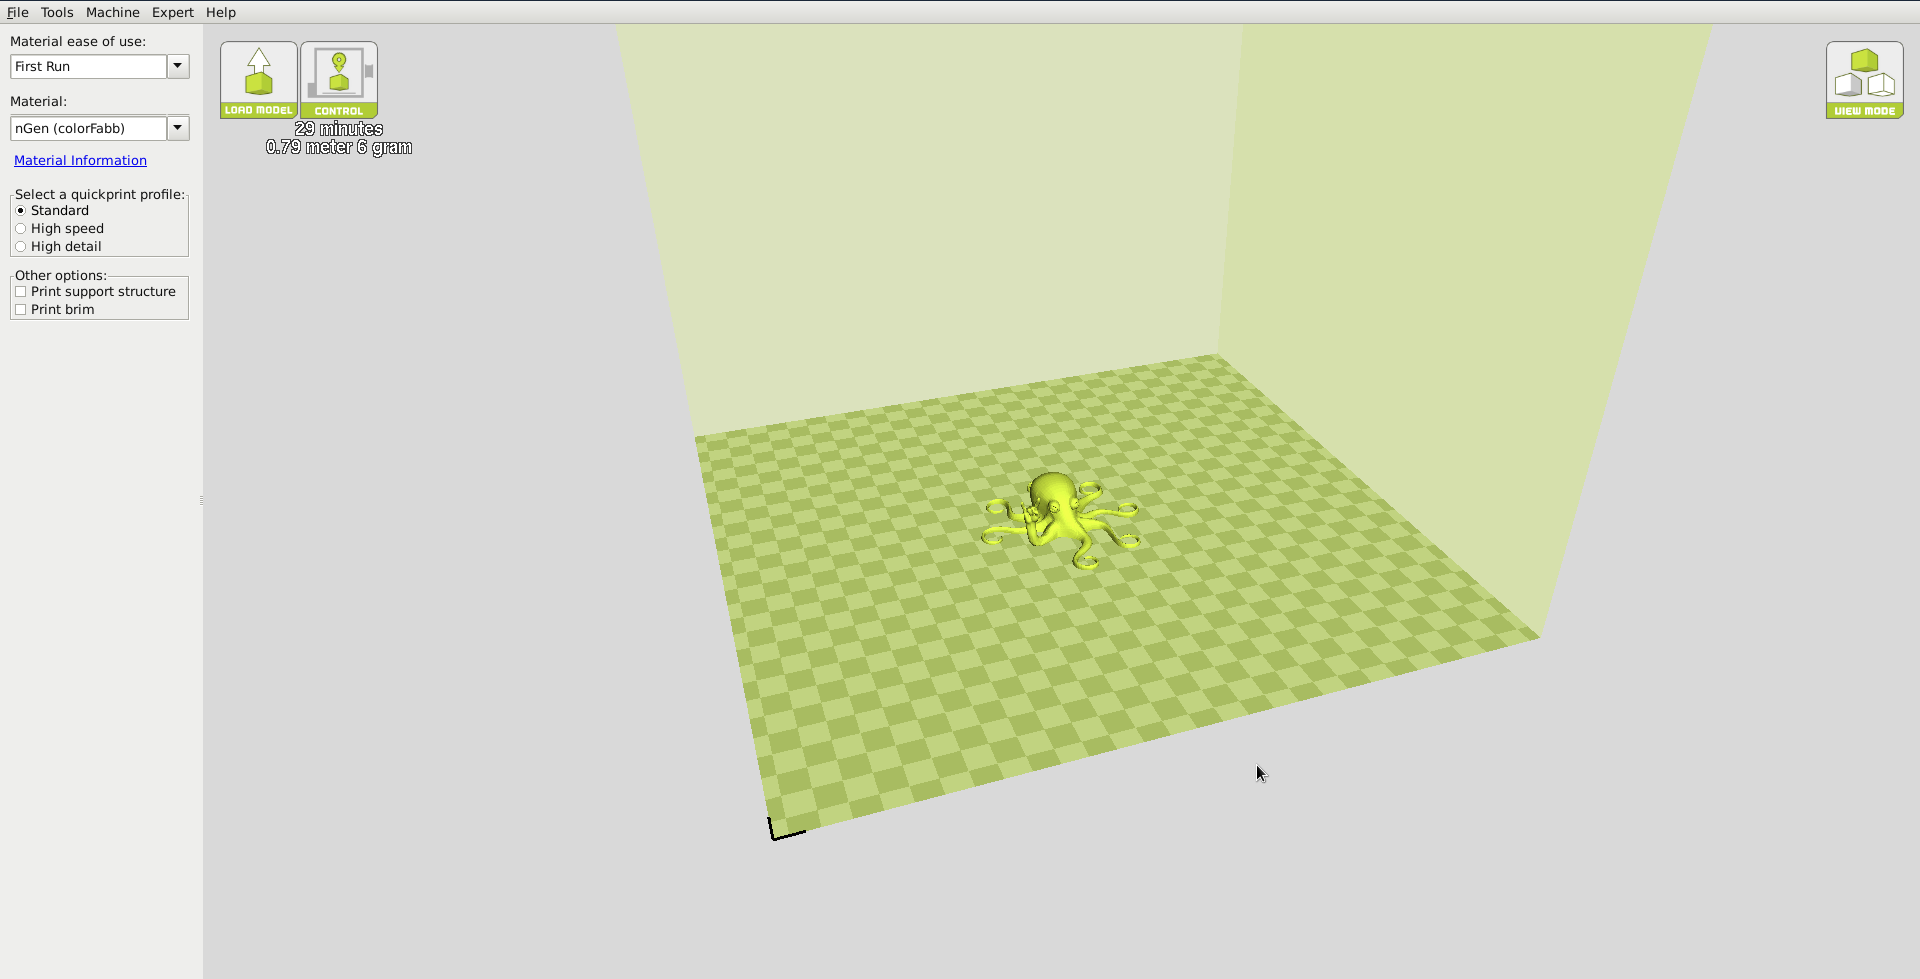
\includegraphics[keepaspectratio=true,angle=0,height=0.4\textheight,width=1.0\textwidth]{quickprintfirstrun.png}
\caption{Quick Print Settings}
\label{fig:Cura}
\end{figure} 
% (photo highlighting profile, material, diameter, and other)
After setting up Cura for the first time, you will be shown the main interface screen. (Fig. \ref{fig:Cura}, page \pageref{fig:Cura}): 

\subsection{Selecting a Quick Print Profile}
\index{Quick Print Profile}
\index{Resolution}
\glossary{Resolution}{In general terms, the resolution you print at can be determined by the layer height you use. The LulzBot\textsuperscript{\miniscule{\texttrademark}} TAZ can print at a layer height of 0.05mm to 0.50mm.}
The print quality settings can be found in the top left-hand corner of the window. For most filaments, there will be Standard, High Speed, and High Detail options. Some of the more exotic filaments may only have a Normal/Standard profile.

\begin{description}
\item[High Detail] \hfill \\
Designed to give greater detail and finer objects. This will have a smaller layer height, which will make each layer thinner, so that curves seem more natural and walls seem less noticeable. This setting will also require more layers to be laid down, increasing overall print time.
\index{High Detail}

\item[Standard] \hfill \\
Designed to give a medium resolution, by increasing the layer height and print speeds. This will make the organic curves slightly more step-like than the fine setting, but will reduce printing time.
\index{Standard Quality}

\item[High Speed] \hfill \\
Designed for the fast prints, where overall model finish is not of concern. Most commonly used for quick iteration of designs found in rapid prototyping.
\index{High Speed}
\end{description}

\subsection{Material Selection}
\index{Material Selection}
\index{filament}
Choose your desired filament. The TAZ ships with a 1 meter sample of ABS, that should be used in your first print.
%If you are not using LulzBot supplied filament, update your filament diameter to your specific average filament diameter. Do this by taking 10 to 12 filament diameter measurements from different parts of the reel and averaging them. Update your filament diameter. You may also want to adjust the temperature, as different manufacturers have different recommended temperatures. % This could be better served in the Full Settings explanation.

\subsection{Printing Support Material}
\index{Support Material}
%%%% Saved for standalone Cura Manual %%%%
%The TAZ and Mini are able to print models that have angles and overhangs, even without support material depending on the overhang distance and angle. Turn this option on if your model could benefit from support material.
%MINI% The Mini 3D printer is able to print models that have angles and overhangs, even without support material depending on the overhang distance and angle. Turn this option on if your model could benefit from support material.
The TAZ 3D printer is able to print models that have angles and overhangs, even without support material depending on the overhang distance and angle. Turn this option on if your model could benefit from support material.

\subsection{Brim}
\index{Brim}
Brim is used to increase surface area of the part you're printing, thereby ensuring proper part adhesion. This will print a single layer high edge around the outside of the part, helping first layer adhesion and minimizing warping.

\subsection{Load Model File}
\index{Load Model}
\index{STL}
Select the STL model you would like to print. Either use the \texttt{Load Model} button or select \texttt{File} > \texttt{Load Model}. Once the file has been loaded, you will see a 3D rendering of your object on the build platform. Select the model to see the various options. 

\subsection{Model Orientation}
\index{Orientation}
Move your model to change where it is printed on the build plate. Do this by left clicking on the model and dragging it to the desired location. The \texttt{black} outlined corner of the 3D print bed view represents the front left hand corner of the build plate on your printer. By holding down the right mouse button and dragging, you can view your model from different angles. %Not sure if this last sentence should be reworked or put in a separate section.
\begin{figure}[H]
\centering
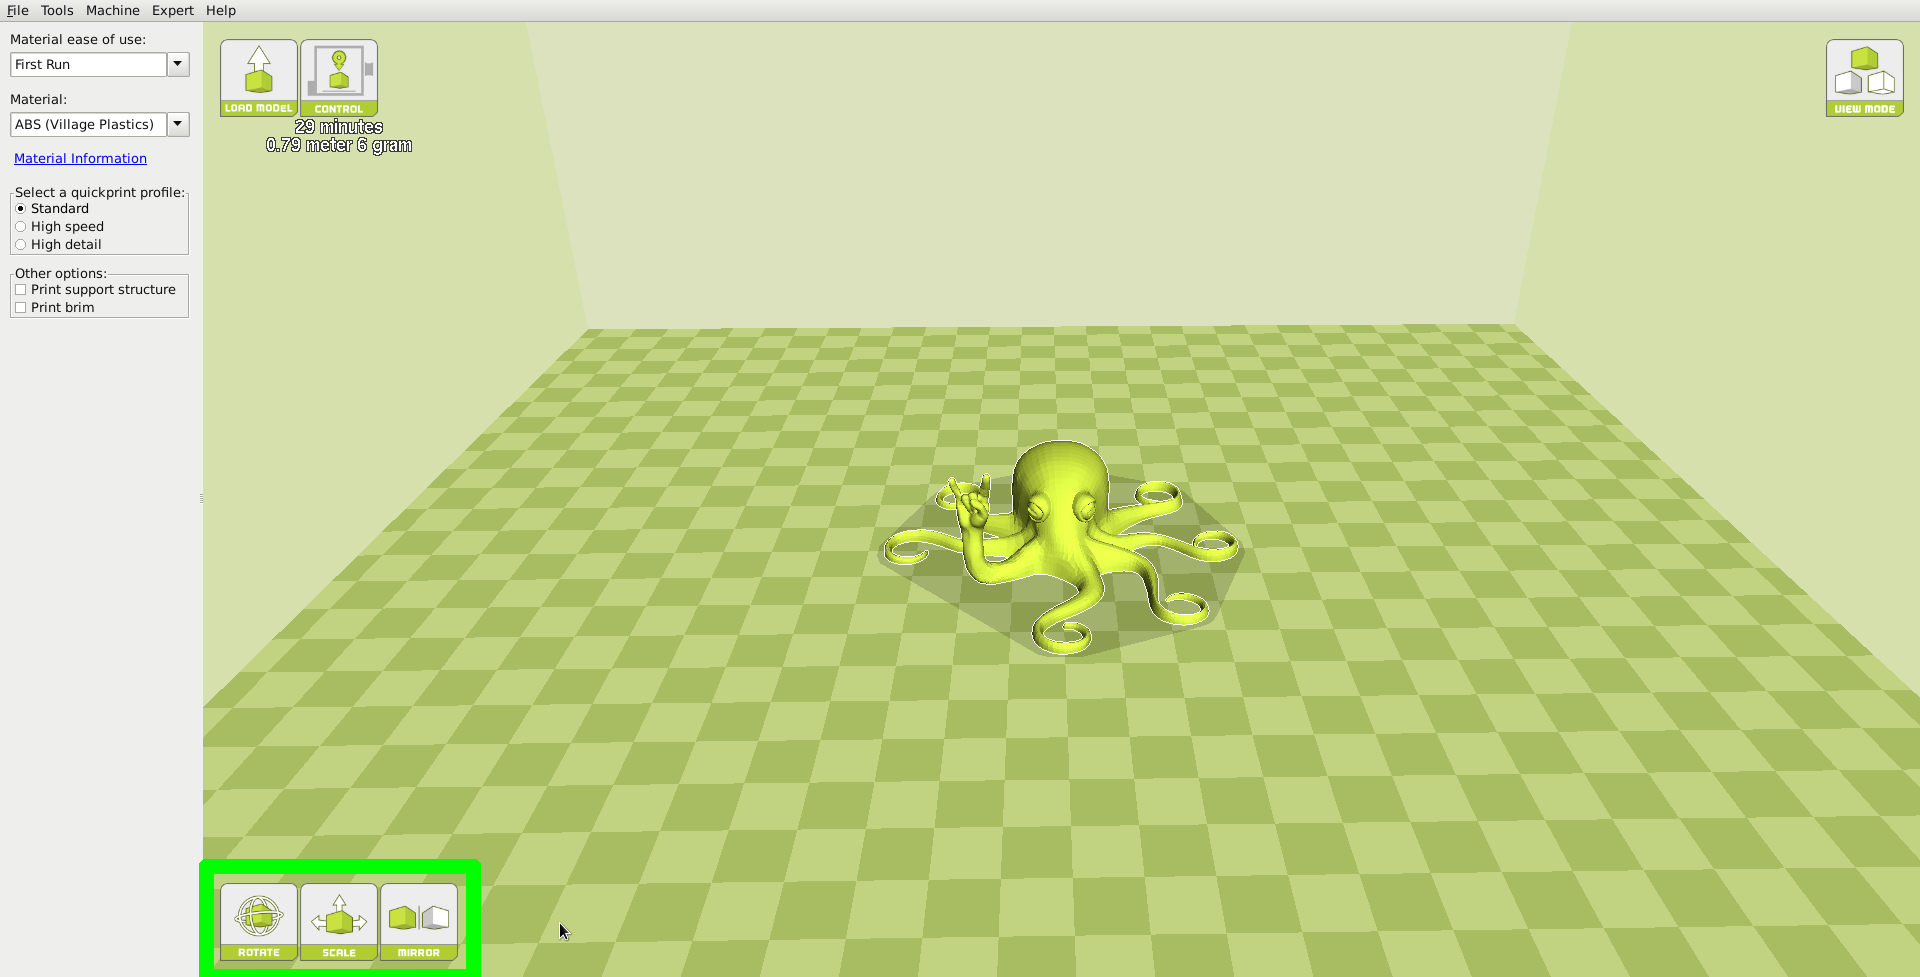
\includegraphics[keepaspectratio=true,angle=0,height=0.4\textheight,width=1.0\textwidth]{optionsTAZ.png}
\caption{Options after selecting model}
\label{fig:Orientation}
\end{figure}

\subsubsection{Rotate}
%%%% Alternate explanation %%%%
%The \texttt{Rotate} button will give you the ability orient your model in along all three axes. Once you click the rotate button, three circles will surround your model. The red circle will allow you to rotate in the XY plane. The Yellow circle will rotate in the XZ plane. The Green circle will rotate in the YZ plane.
\definecolor{yellow1}{cmyk}{0,0,1,0.30}
\definecolor{green1}{rgb}{0.30,1,0.30}
The \texttt{Rotate} button will give you the ability to orient your model in along all three axes. Once you click the rotate button, three circles will surround your model. The \textcolor{red}{red circle} will allow you to rotate around the \textcolor{red}{Z axis}. The \textcolor{yellow1}{Yellow circle} will rotate around the \textcolor{yellow1}{Y axis}. The \textcolor{green1}{Green circle} will rotate around the \textcolor{green}{X axis}. Cura defaults to 15 degree increments. Hold \texttt{Shift} to rotate by \texttt{One Degree Increments}.
\begin{figure}[H]
\centering
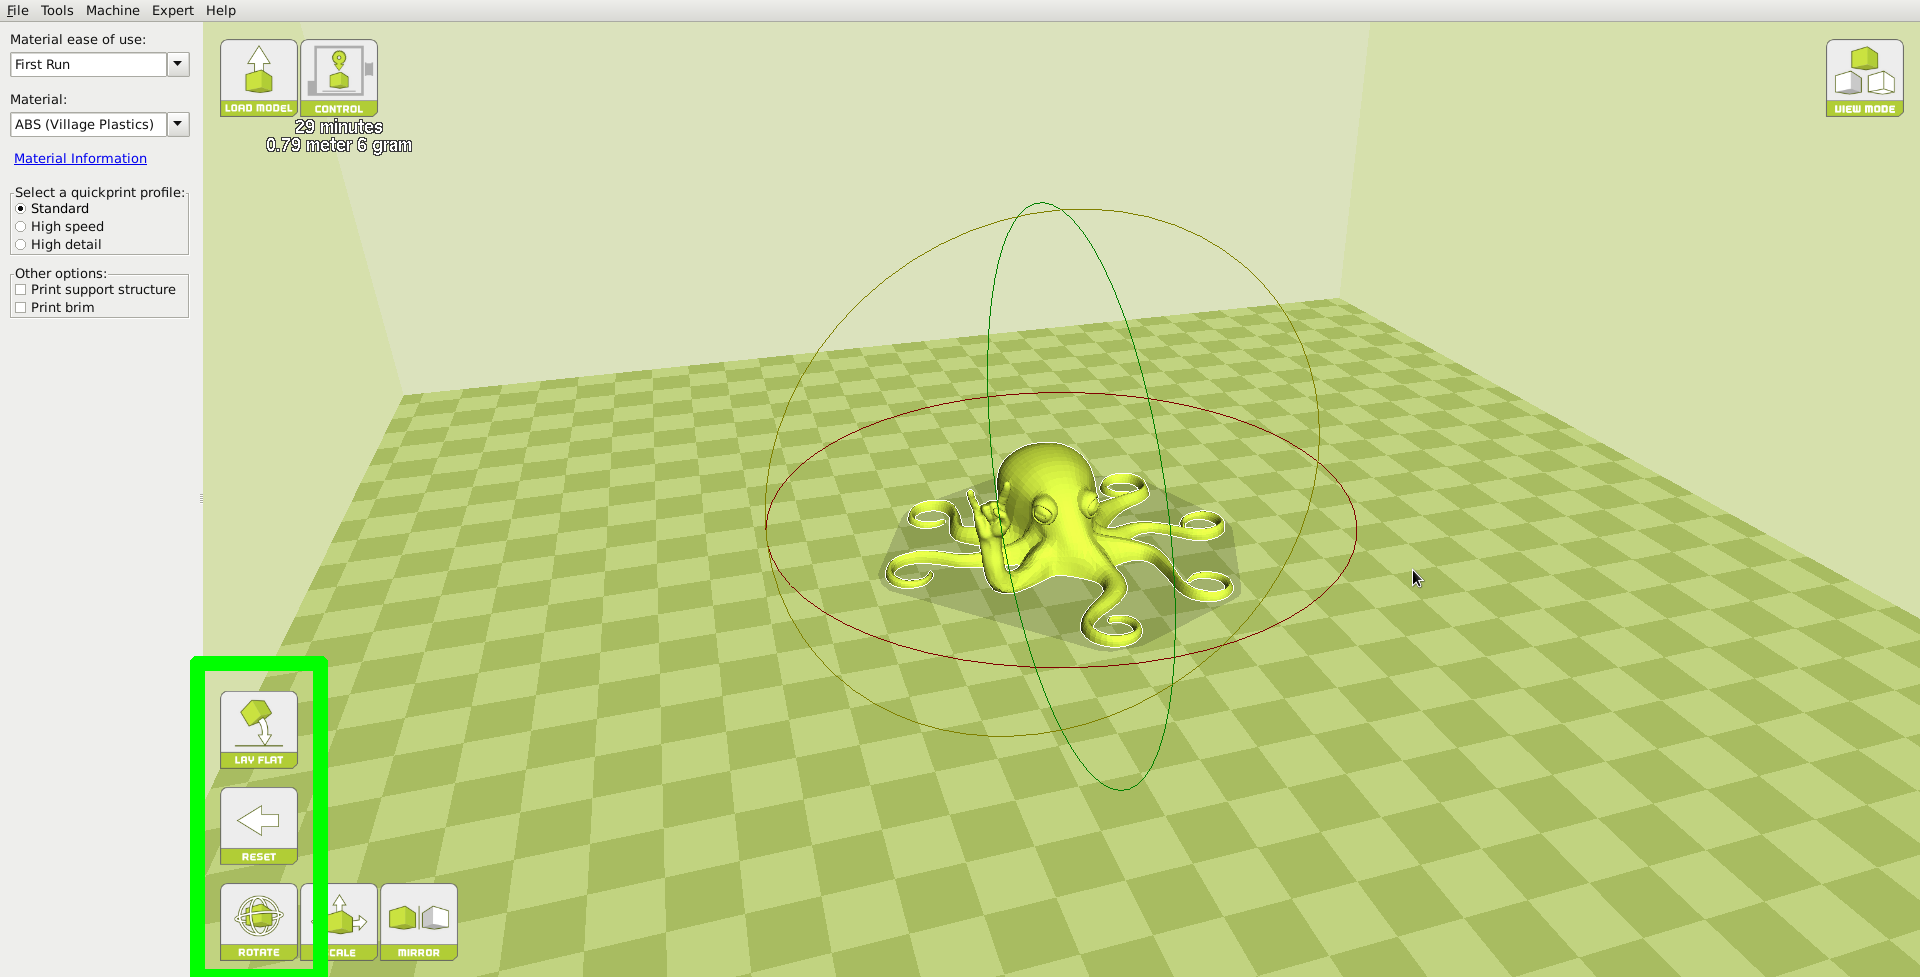
\includegraphics[keepaspectratio=true,angle=0,height=0.4\textheight,width=1.0\textwidth]{rotateTAZ.png}
\caption{Rotating your Model}
\label{fig:Rotating your Model}
\end{figure}

\subsubsection{Lay Flat}
The \texttt{Lay Flat} button will ensure that the flat portion of your print is securely attached to the bed. It is highly recommended to use this option after rotating your model in the Z direction, as it will help prevent adhesion issues during the print.
%\begin{figure}[hbt]
%\centering
%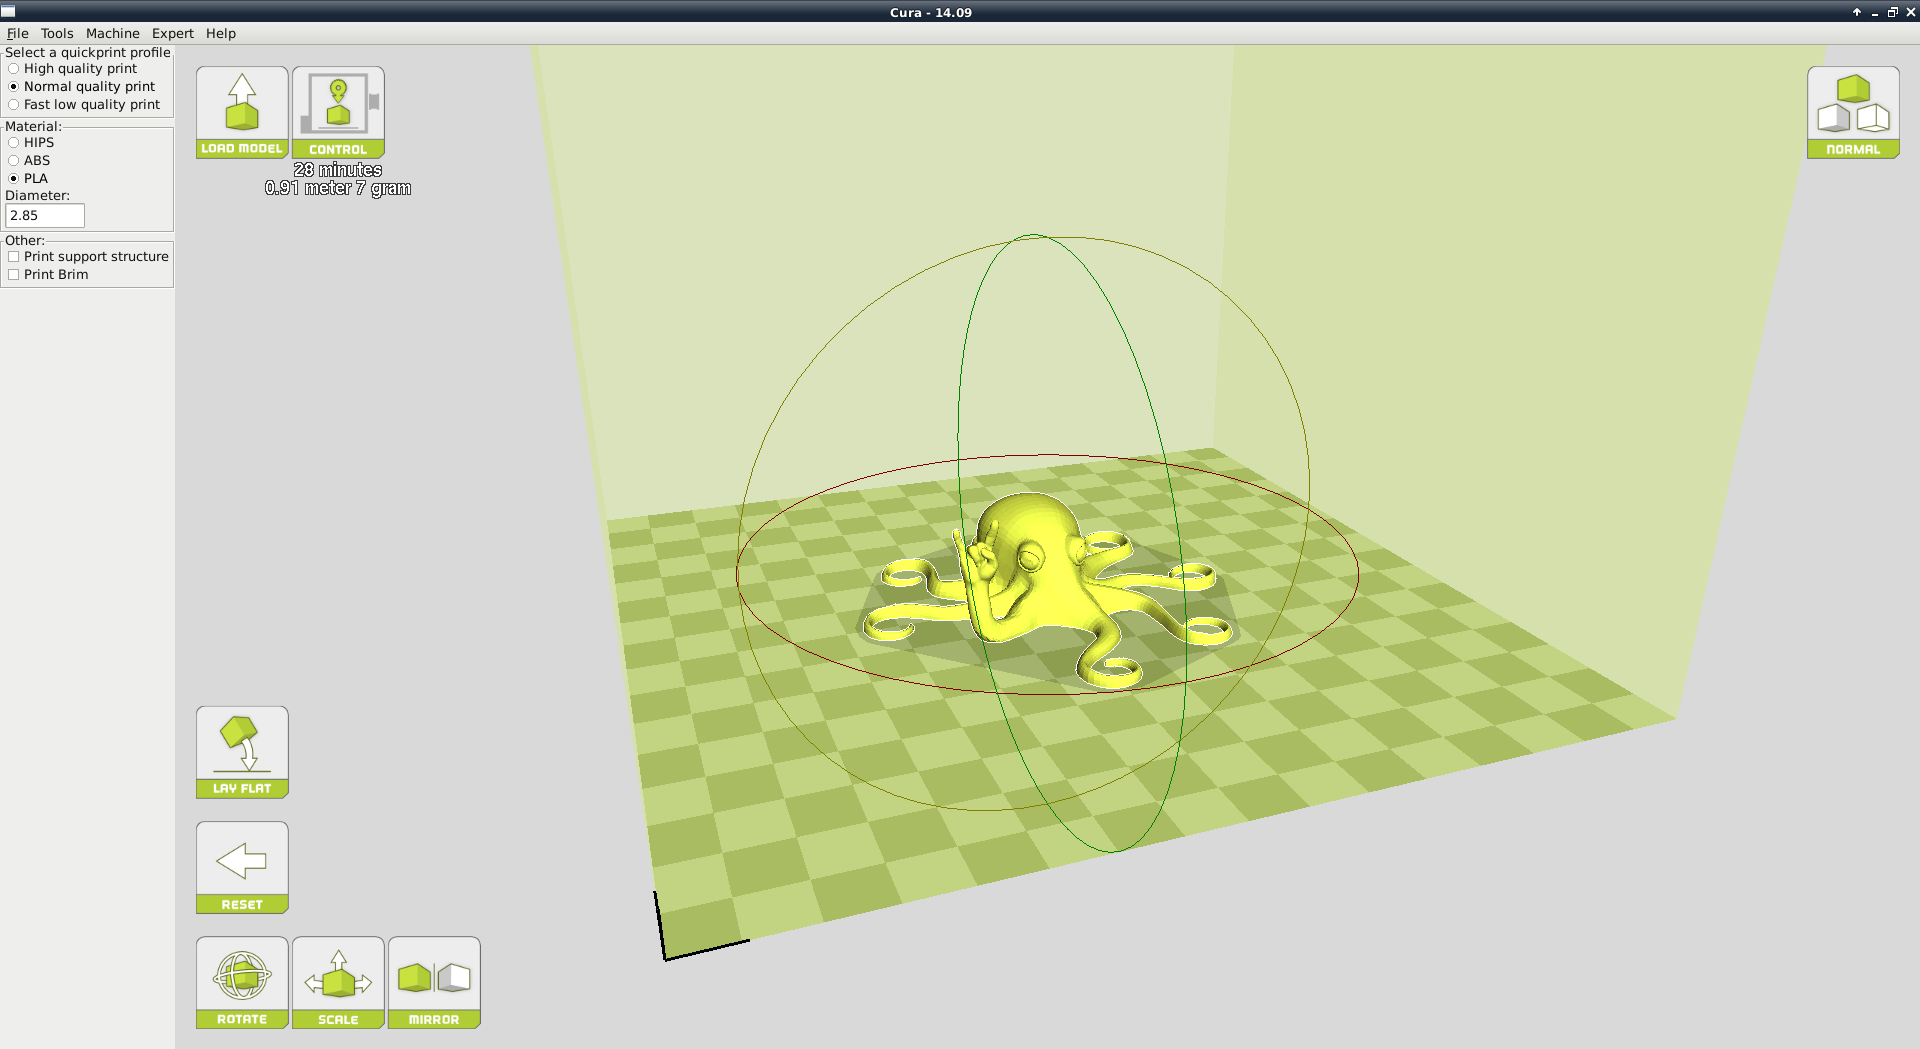
\includegraphics[keepaspectratio=true,angle=0,height=0.4\textheight,width=1.0\textwidth]{Rotate.png}
%\caption{Rotating your Model}
%\label{fig:Rotating your Model}
%\end{figure}

\subsubsection{Reset}
The \texttt{Reset} button will return your model to the original orientation as defined by the CAD program used to create the model.
%\begin{figure}[hbt]
%\centering
%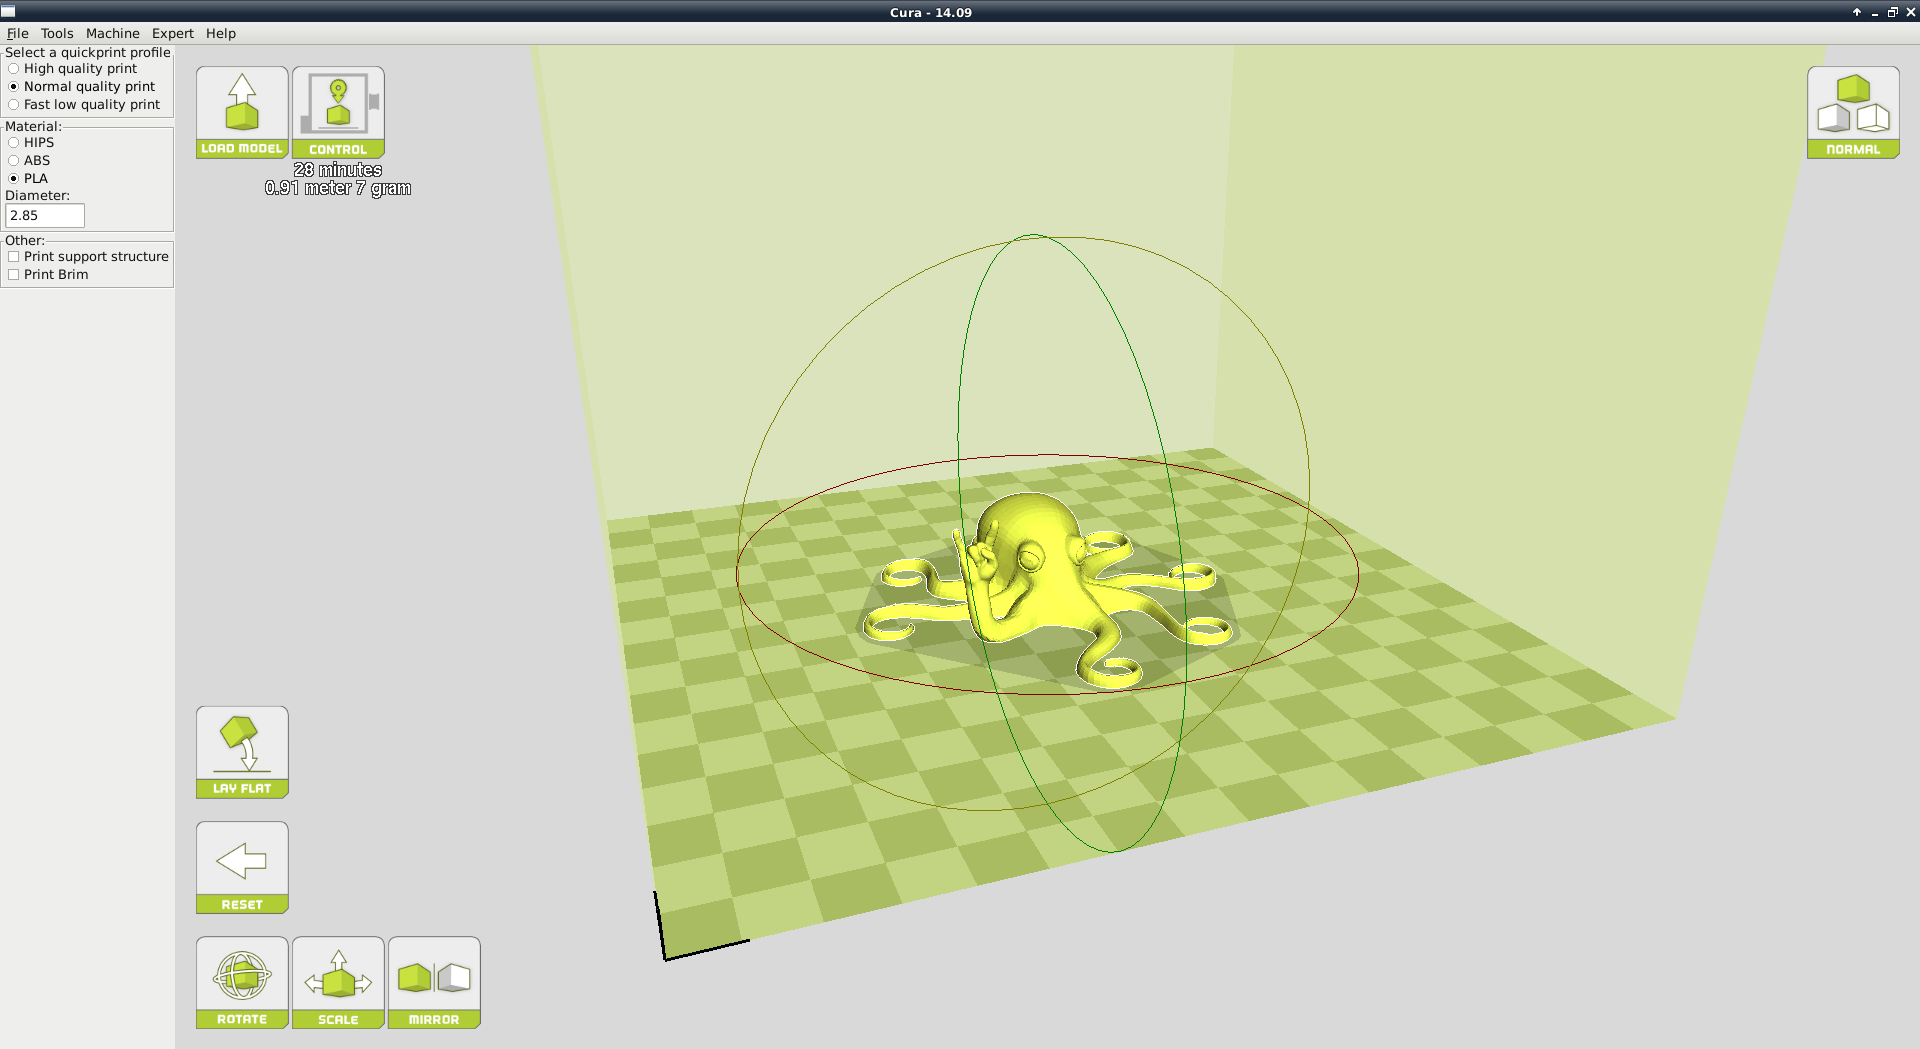
\includegraphics[keepaspectratio=true,angle=0,height=0.4\textheight,width=1.0\textwidth]{Rotate.png}
%\caption{Rotating your Model}
%\label{fig:Rotating your Model}
%\end{figure}

\subsubsection{Scale}
The \texttt{Scale} button displays the model dimensions, along with the ability to scale along the X Y or Z axes. Anything \texttt{below} the number \texttt{1.0} will reduce the objects size, while anything \texttt{above} the number \texttt{1.0} will increase the objects size. As a default, it will be set to uniform scaling. This will cause the X Y and Z axes to be scaled by the same amount when you make a change to any of them. To disable this, select the lock in the lower section of the scaling window. 
\begin{figure}[H]
\centering
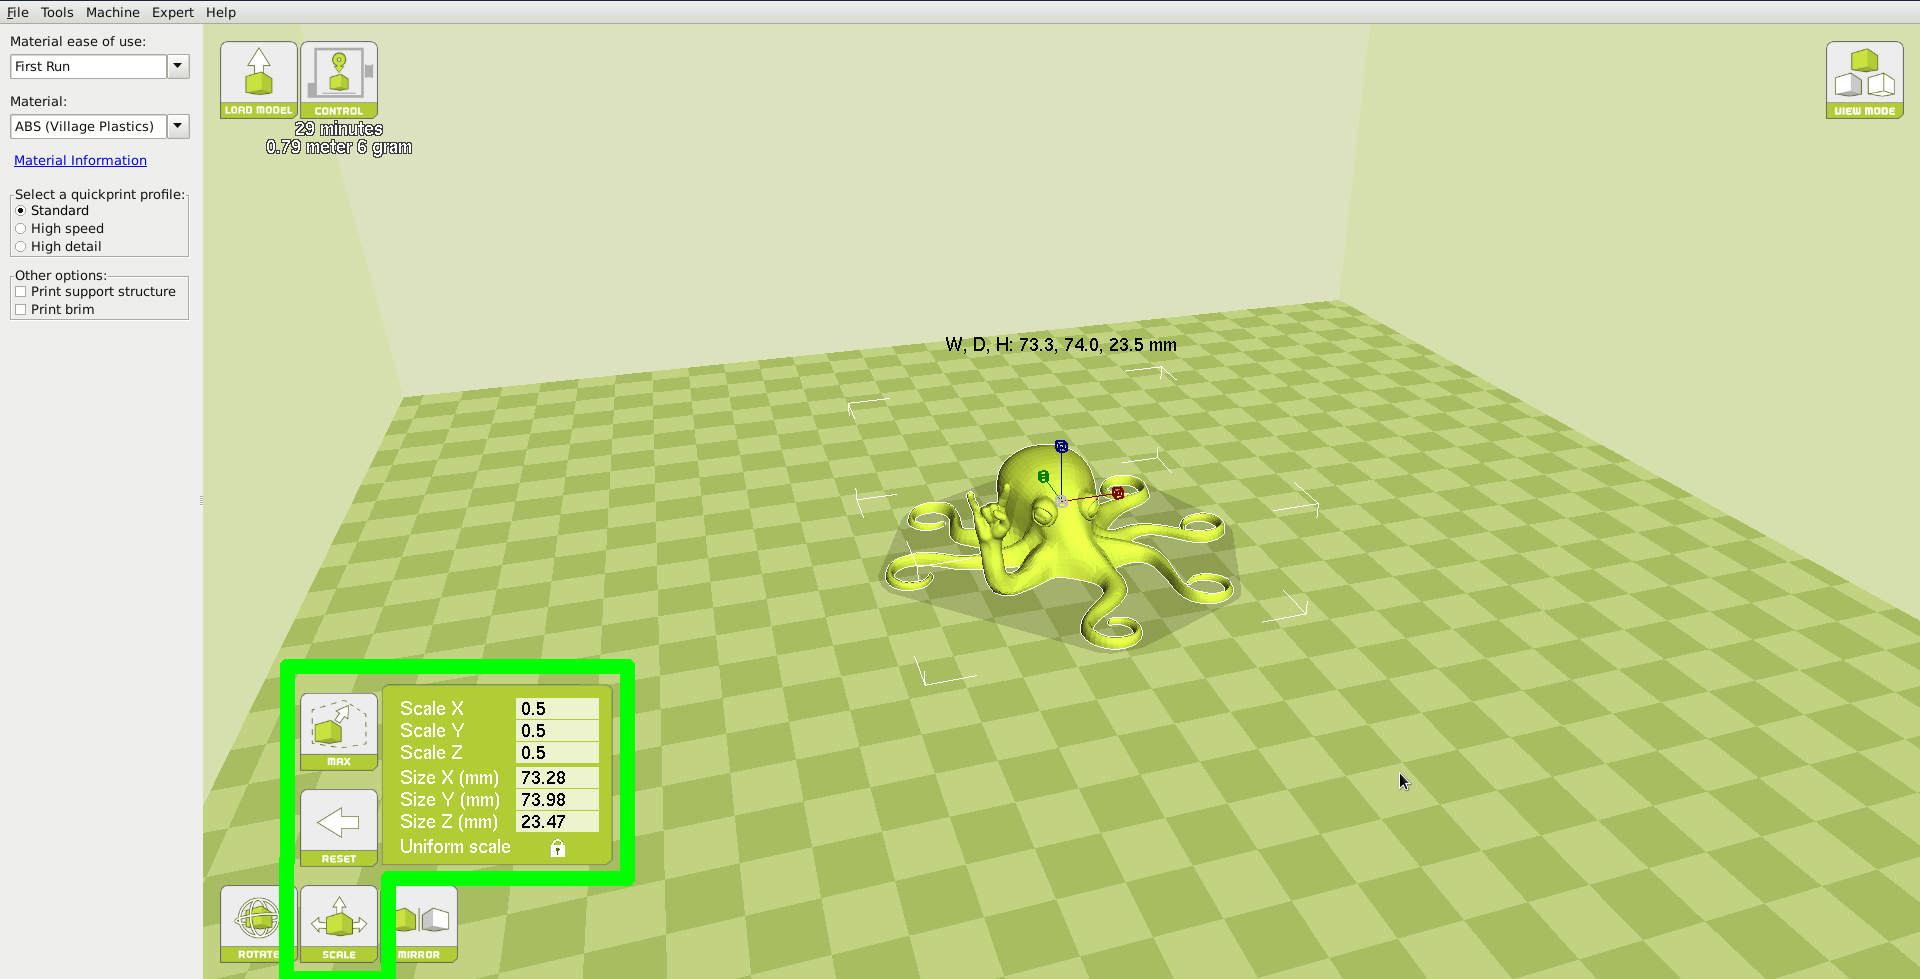
\includegraphics[keepaspectratio=true,angle=0,height=0.4\textheight,width=1.0\textwidth]{scaleTAZ.png}
\caption{Scaling your Model}
\label{fig:Scaling your Model}
\end{figure}

\section{View Options}
\index{View Options}
This mode allows you to view your model in a variety of different ways. This can be helpful for spotting issues before the print even starts. 

\subsection{Normal}
This is the standard view and shows the solid outer surfaces of the model. (Fig. \ref{fig:Normal View}, page \pageref{fig:Normal View}): 

\begin{figure}[H]
\centering
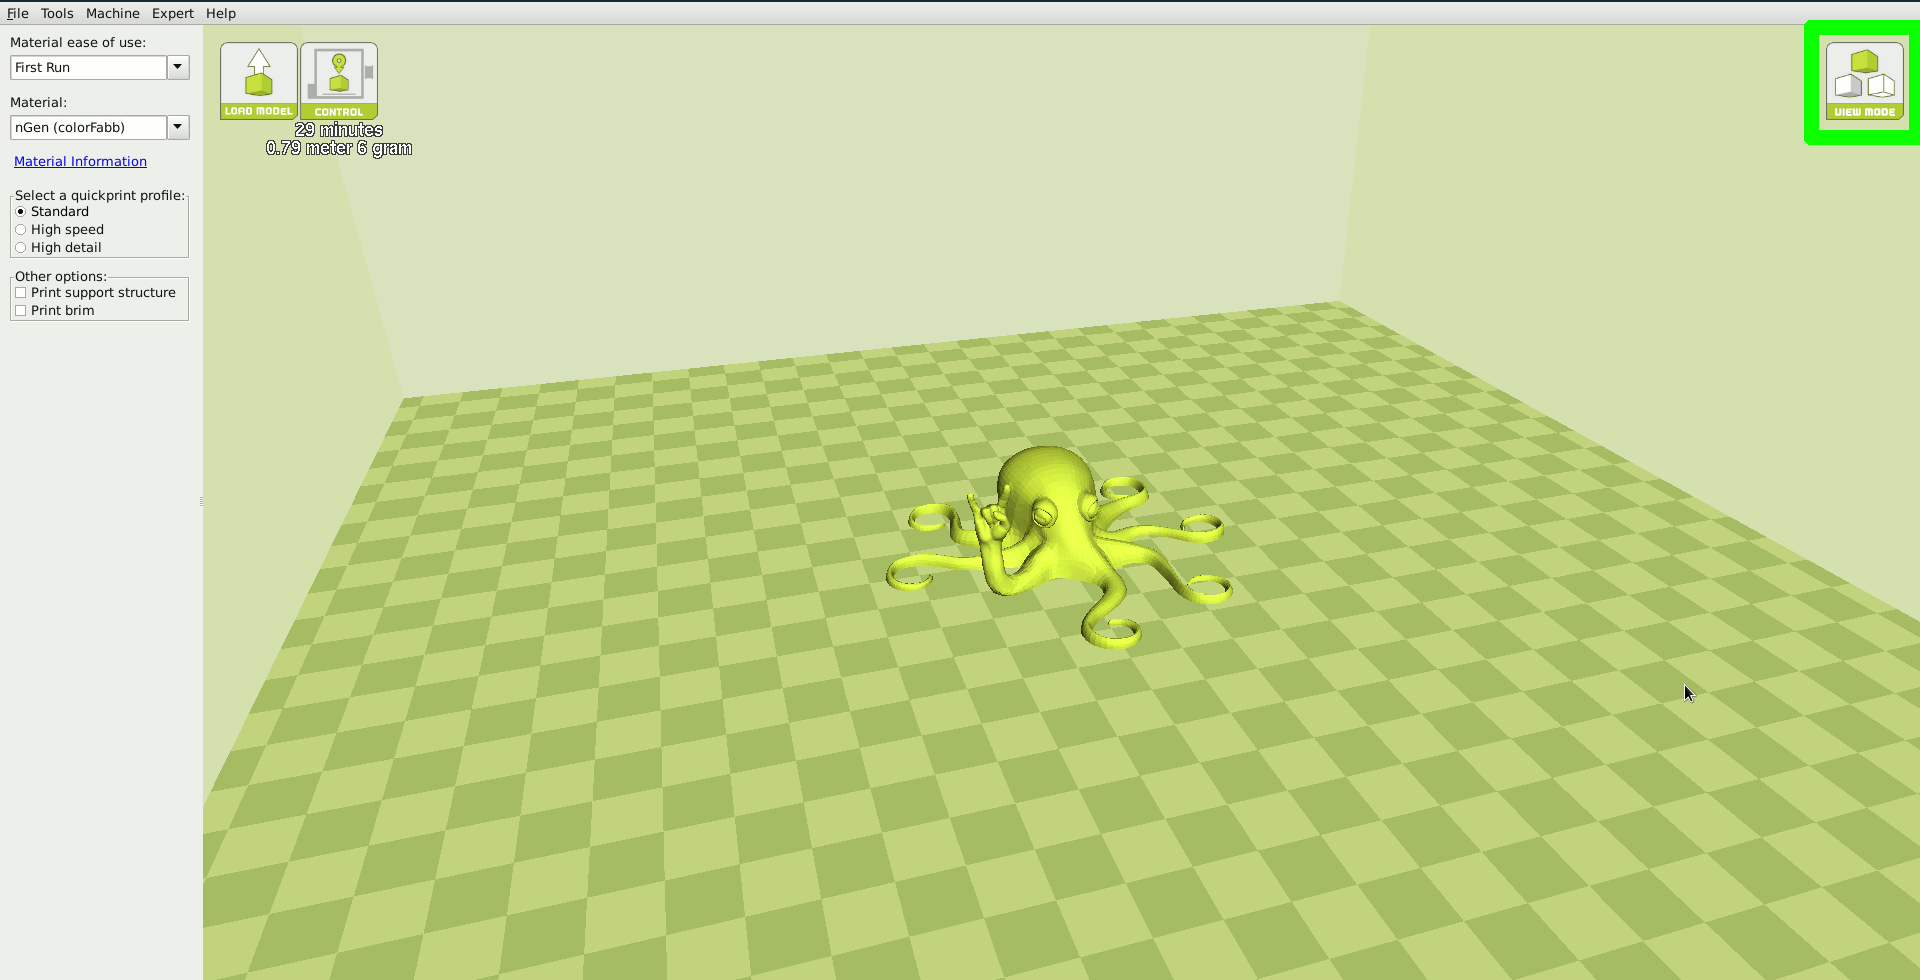
\includegraphics[keepaspectratio=true,angle=0,height=0.3\textheight,width=1.0\textwidth]{viewTAZ.png}
\caption{View in Normal Mode}
\label{fig:Normal View}
\end{figure}

\subsection{Overhang}
\index{Overhang} 
Overhang mode shows where your model may need support material. In Fig. \ref{fig:Overhang_View}, page \pageref{fig:Overhang_View} the red highlighted areas show overhangs and more severe angles and areas where support material is recommended. The overhang threshold can be defined in Expert Settings.
\begin{figure}[H]
\centering
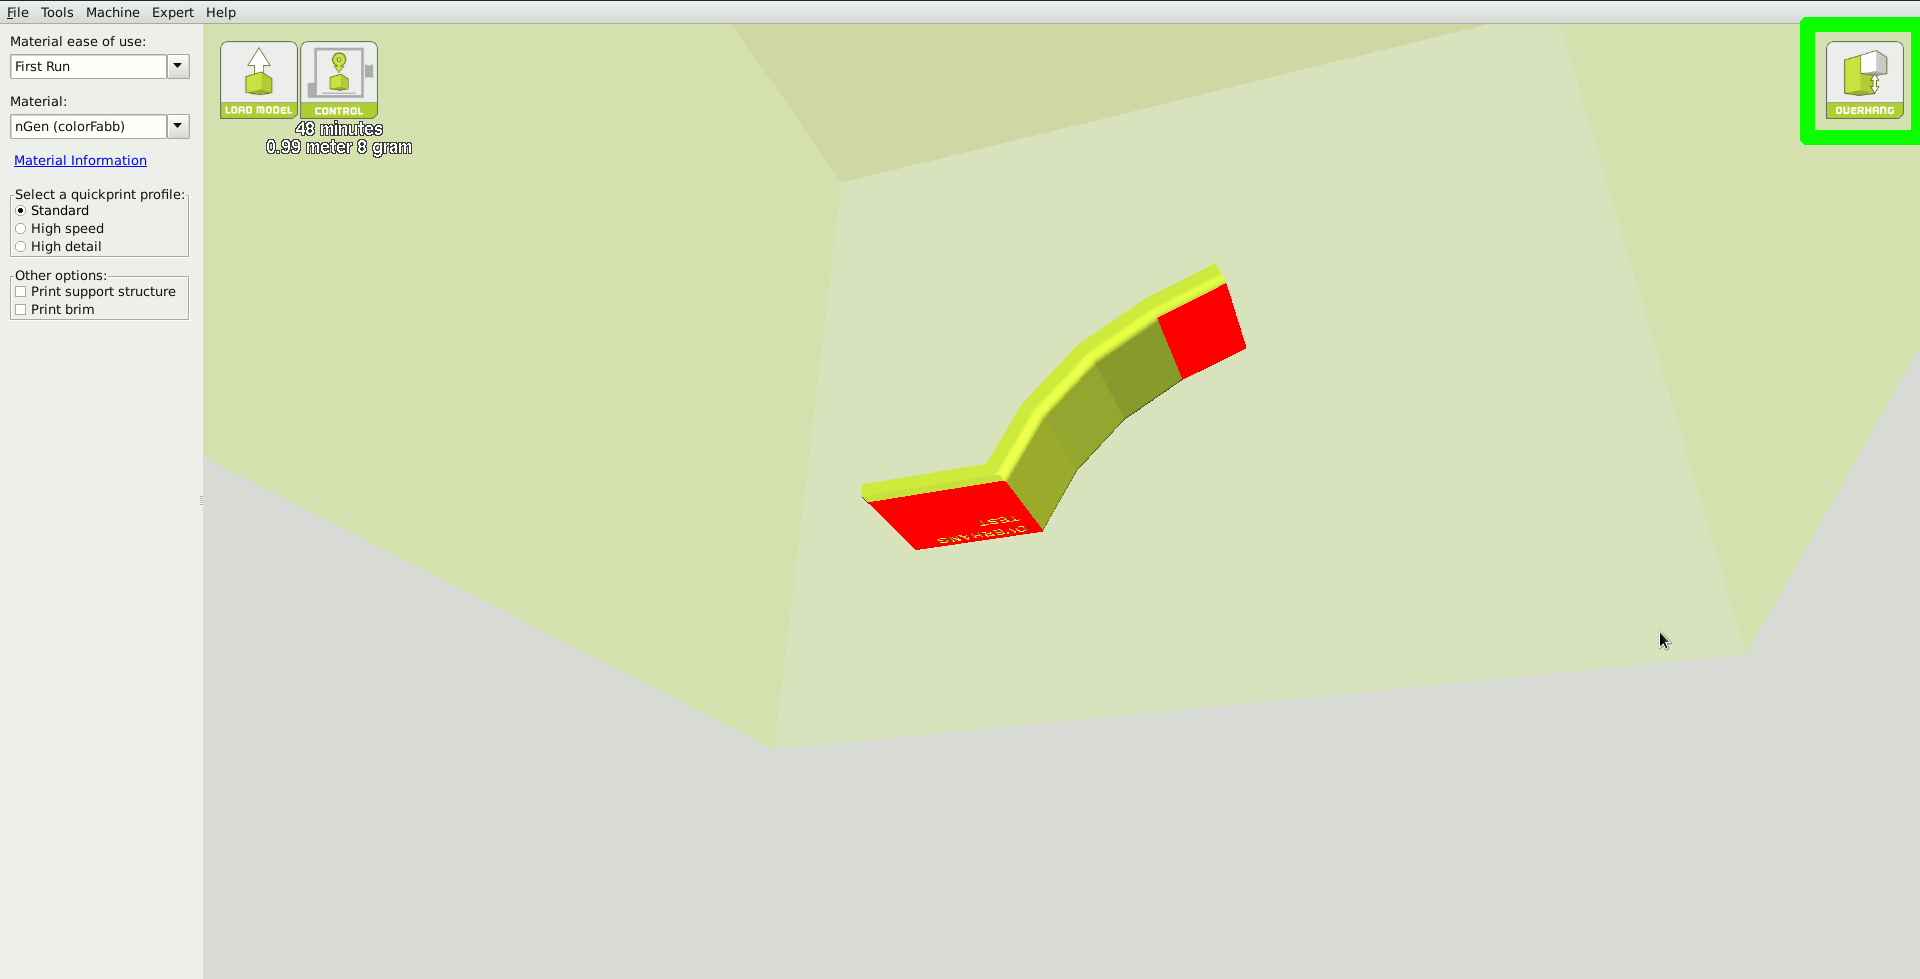
\includegraphics[keepaspectratio=true,angle=0,height=0.3\textheight,width=1.0\textwidth]{overhangTAZ.png}
\caption{View in Overhang}
\label{fig:Overhang_View}
\end{figure}

\subsection{Ghost}
\index{Ghost}
Ghost view mode makes the model translucent to allow you to see what is behind it.
\begin{figure}[H]
\centering
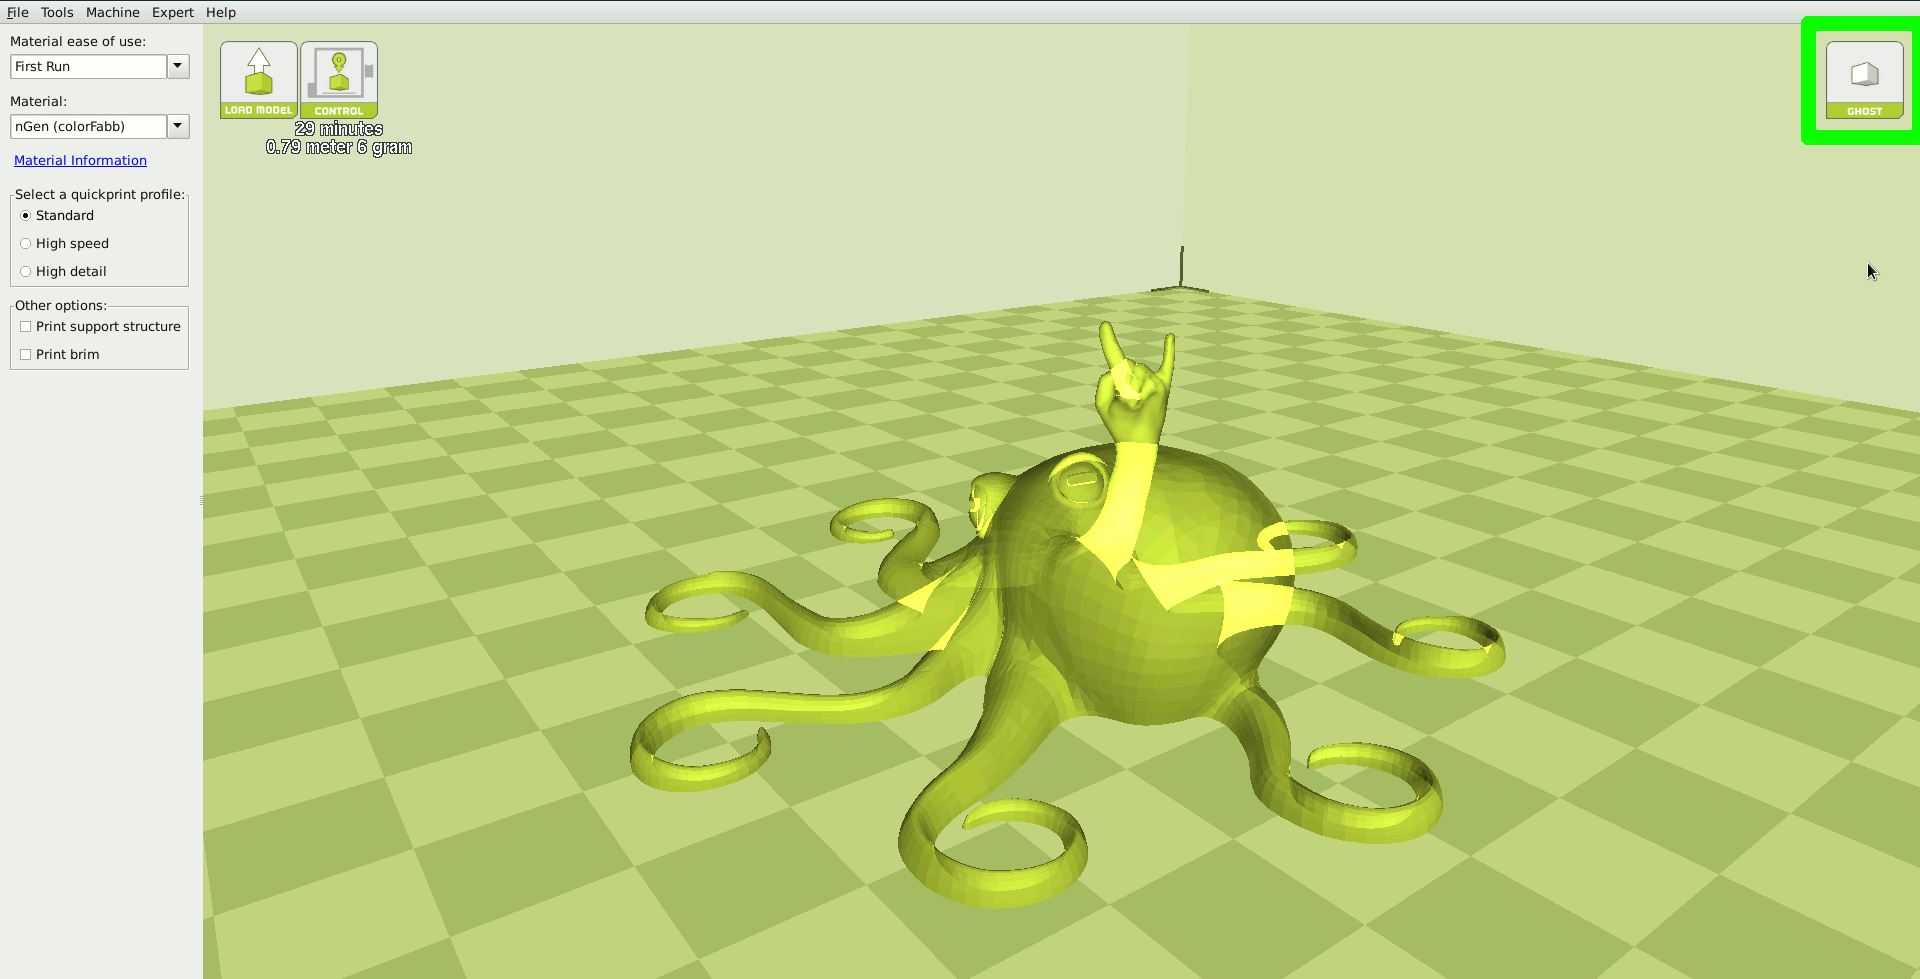
\includegraphics[keepaspectratio=true,angle=0,height=0.3\textheight,width=1.0\textwidth]{ghostTAZ.png}
\caption{View in Ghost}
\label{fig:Ghost View}
\end{figure}

\subsection{Xray}
\index{Xray}
Xray is very similar to Ghost mode. It will allow you to see into objects, ensuring that inner details are correct.
\begin{figure}[H]
\centering
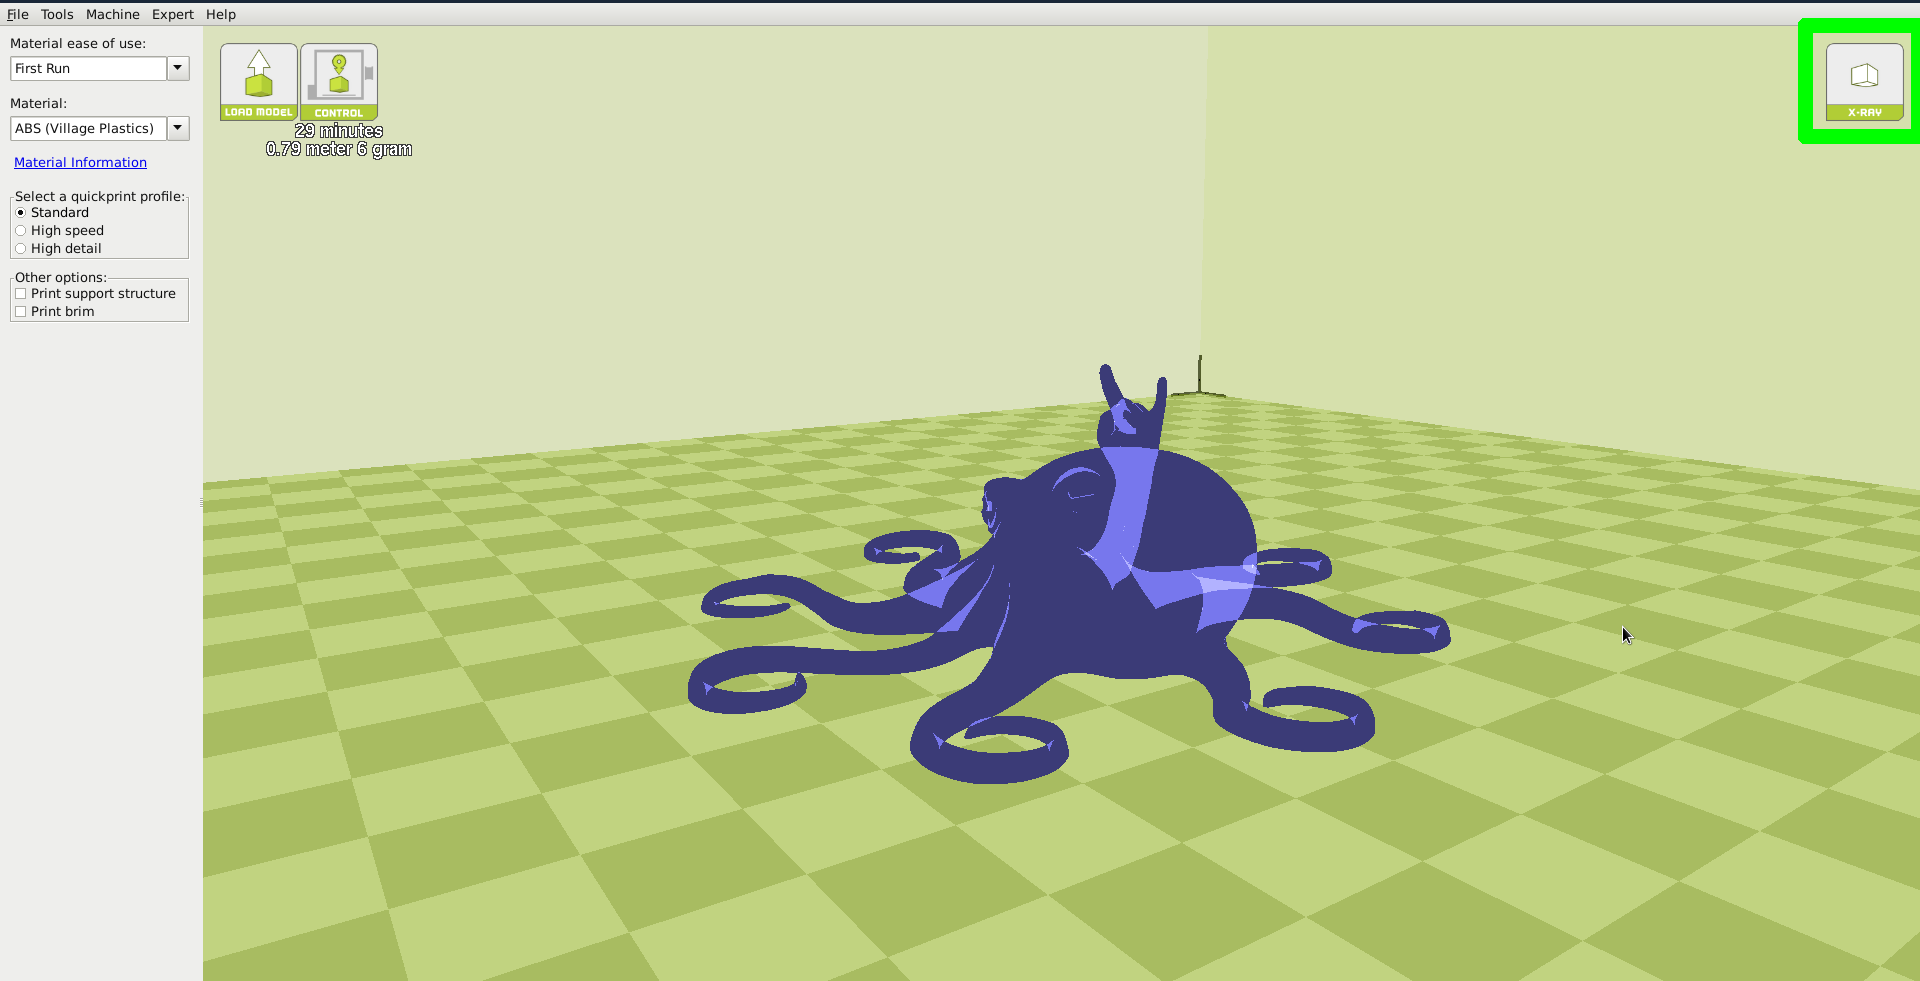
\includegraphics[keepaspectratio=true,angle=0,height=0.3\textheight,width=1.0\textwidth]{xrayTAZ.png}
\caption{View in Xray}
\label{fig:Xray View}
\end{figure}

\subsection{Layers}
\index{Layers}
To view the tool path of your print head and to ensure no skipped layers or gaps use this option. Use the slide bar on the right hand side of the window to move up and down through the tool path layers. Click the icon below it to view an individual layer at a time. If there is support activated in your model, it will be shown in blue.
\begin{figure}[H]
\centering
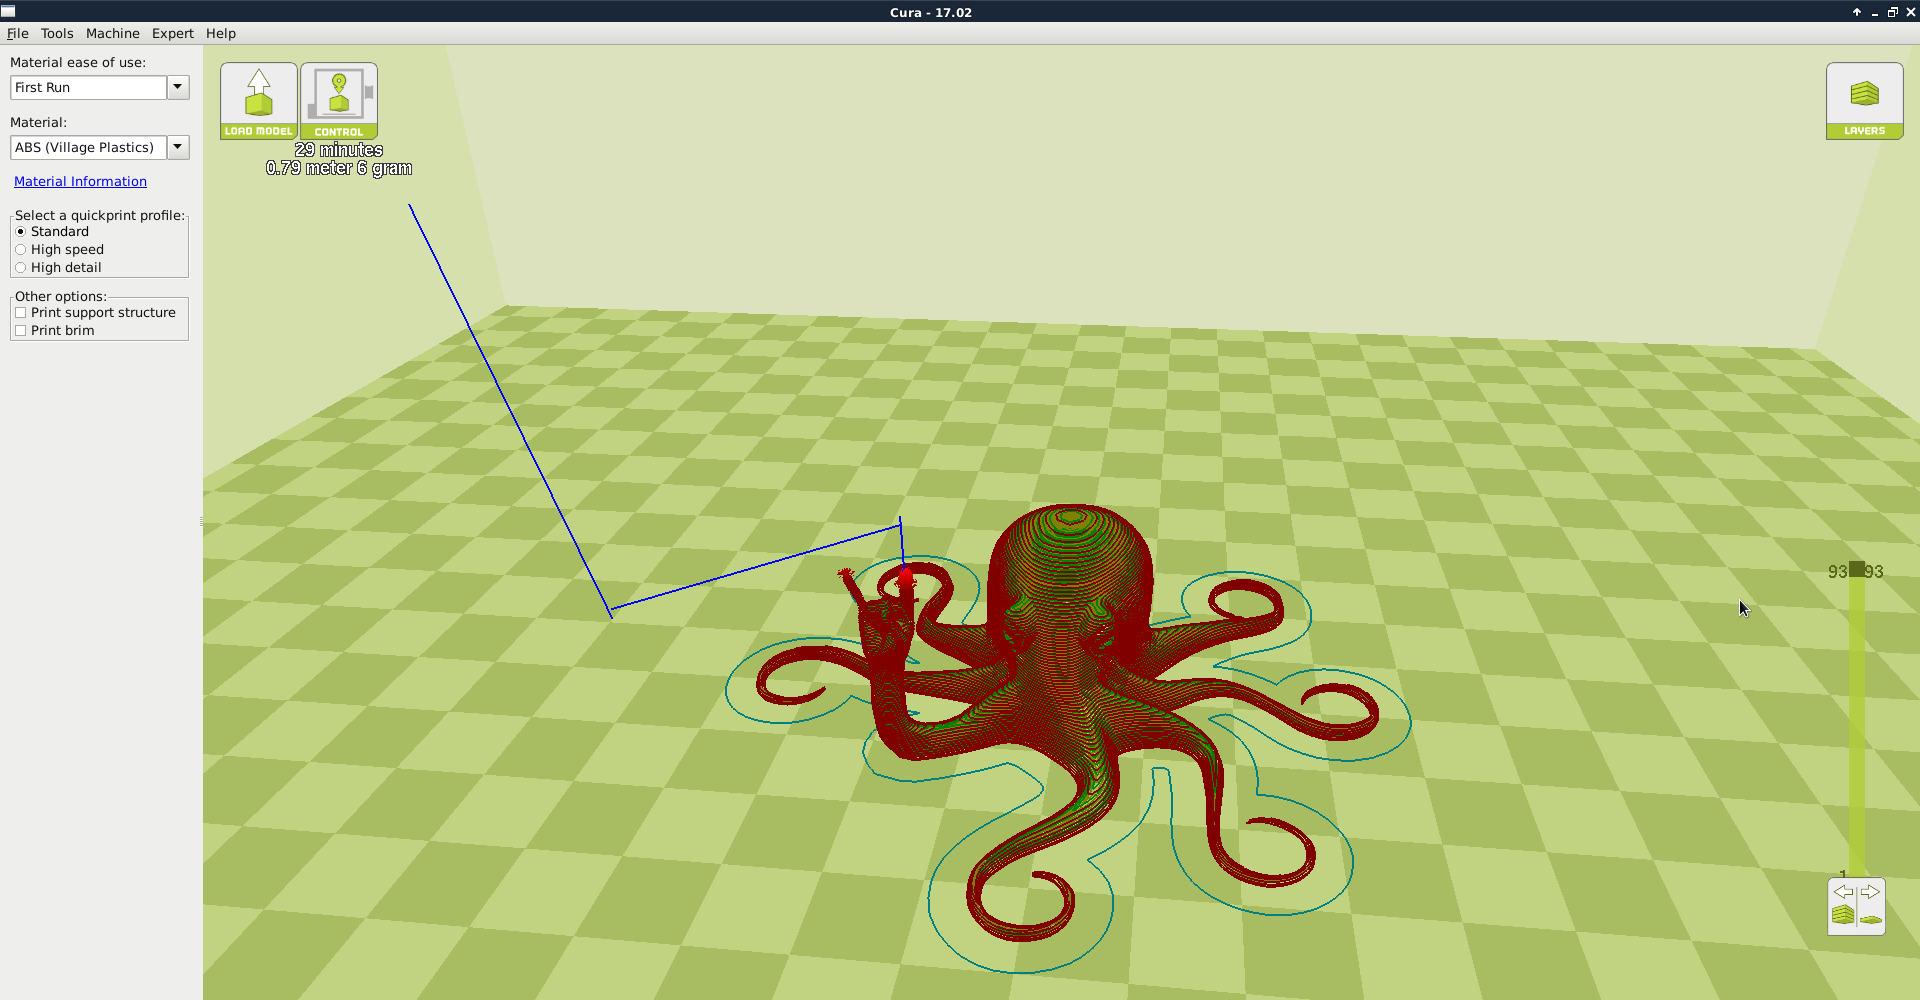
\includegraphics[keepaspectratio=true,angle=0,height=0.3\textheight,width=1.0\textwidth]{layersTAZ.png}
\caption{View in Layers}
\label{fig:Layers View}
\end{figure}

\begin{figure}[H]
\centering
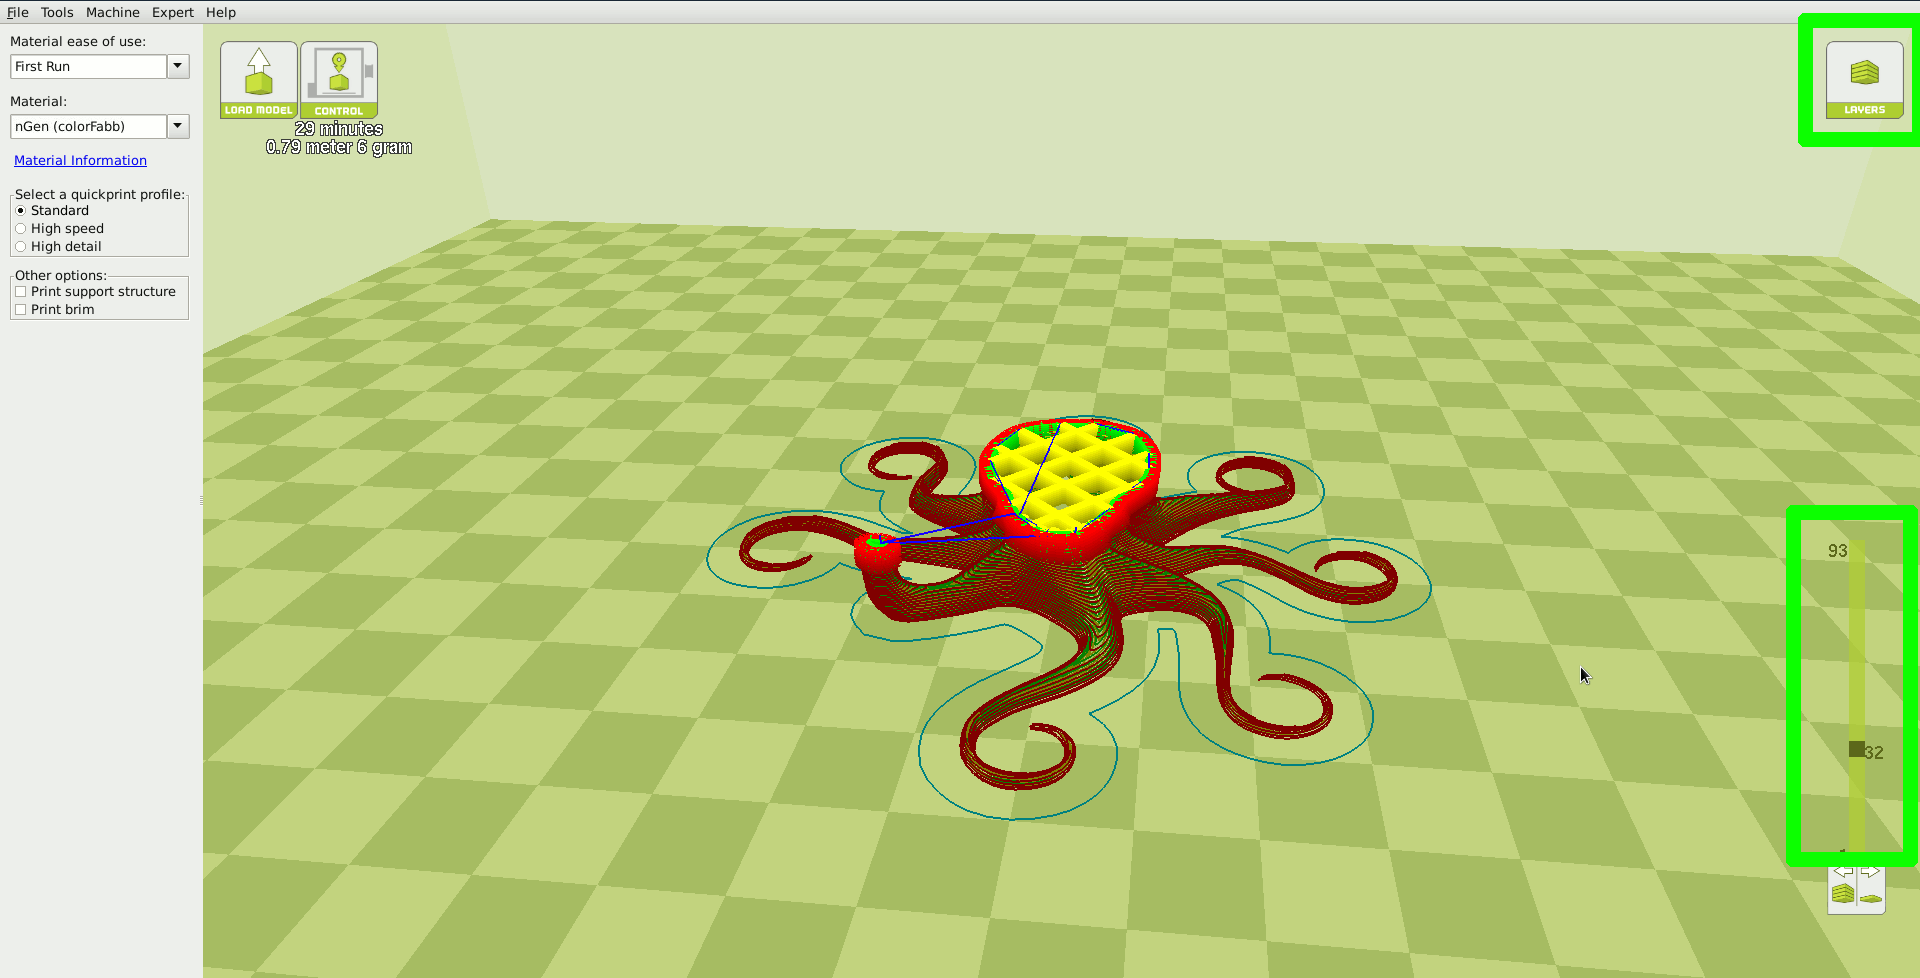
\includegraphics[keepaspectratio=true,angle=0,height=0.3\textheight,width=1.0\textwidth]{cumulativeTAZ.png}
\caption{Viewing Cumulative Layers}
\label{fig:Mid Layers View}
\end{figure}

\begin{figure}[H]
\centering
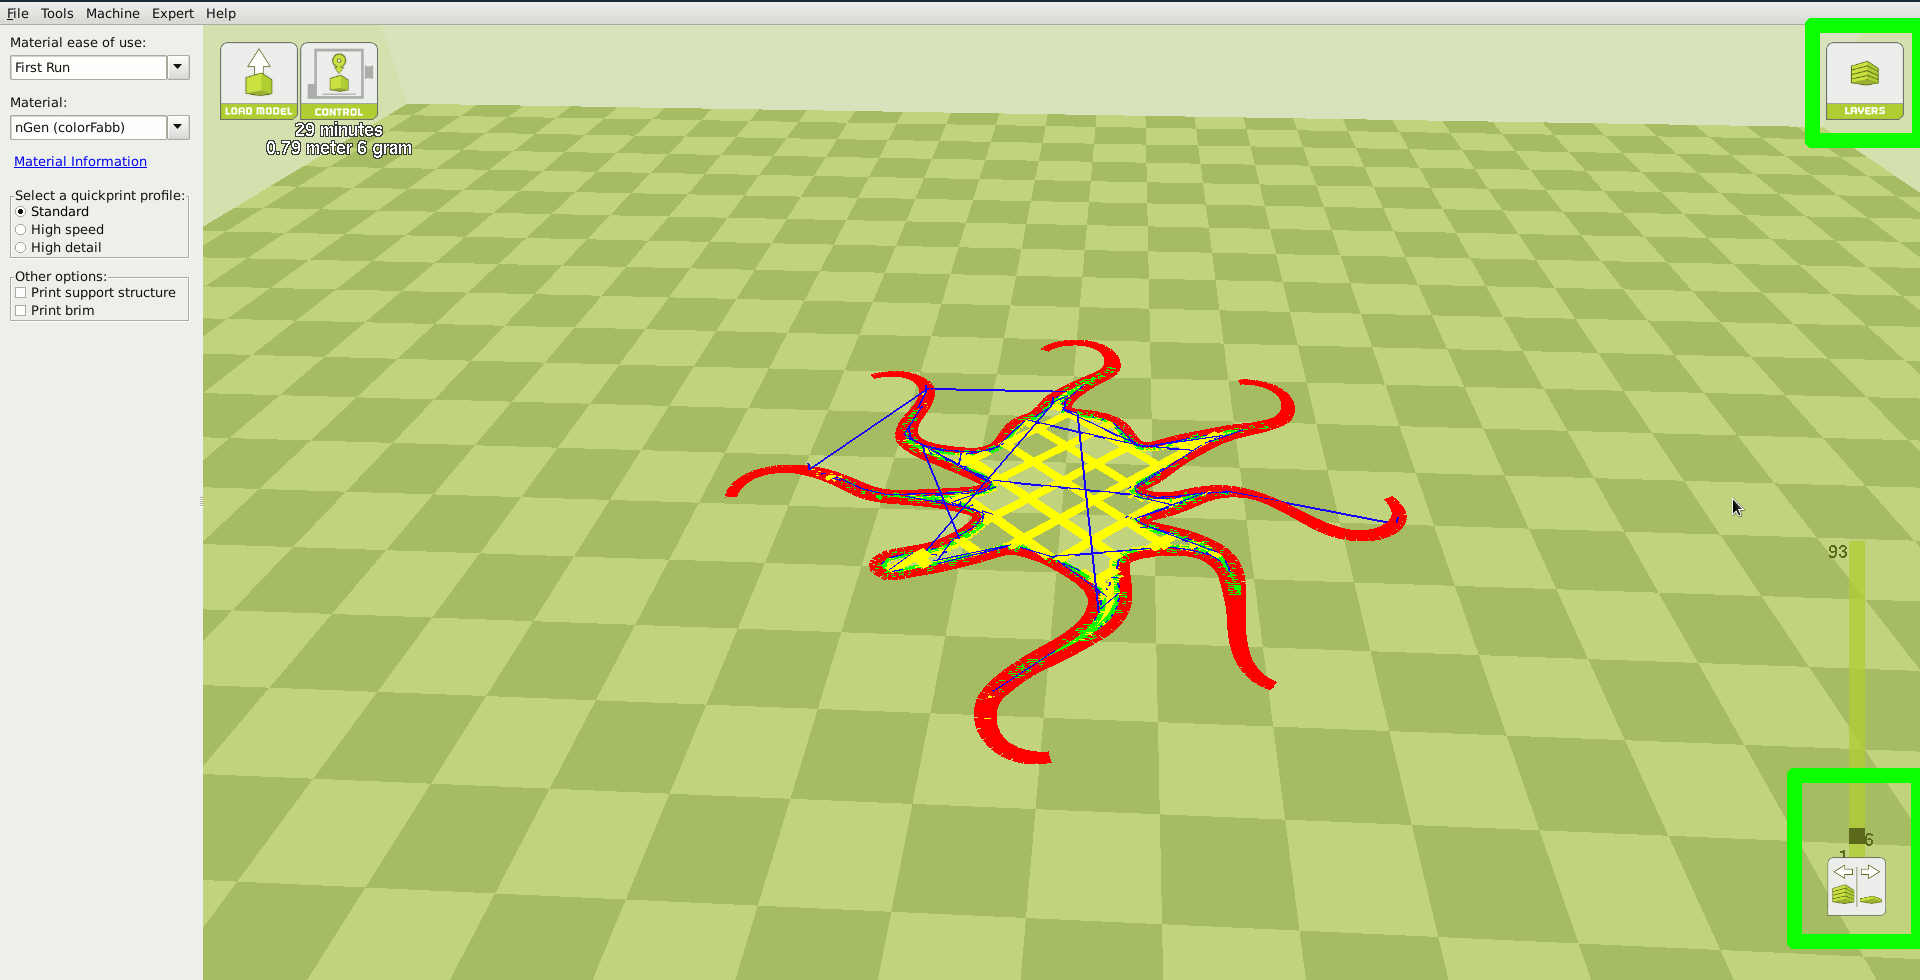
\includegraphics[keepaspectratio=true,angle=0,height=0.3\textheight,width=1.0\textwidth]{individualTAZ.png}
\caption{Viewing Specific Layers}
\label{fig:Viewing Specific Layer}
\end{figure}

\section{Starting Your First Print}
\index{First Print}
Once you have your model, profile, and filament loaded, it is time for your first print! 


%\subsection{Mini}

%Select the \texttt{Print/Control} option in the top left hand corner of your build volume. This will bring up your Printer Interface. Please wait for the window title to display \texttt{operational} before sending any commands to the printer..

%\pageref{fig:Print Control}).
%\begin{figure}[hbt]
%\centering
%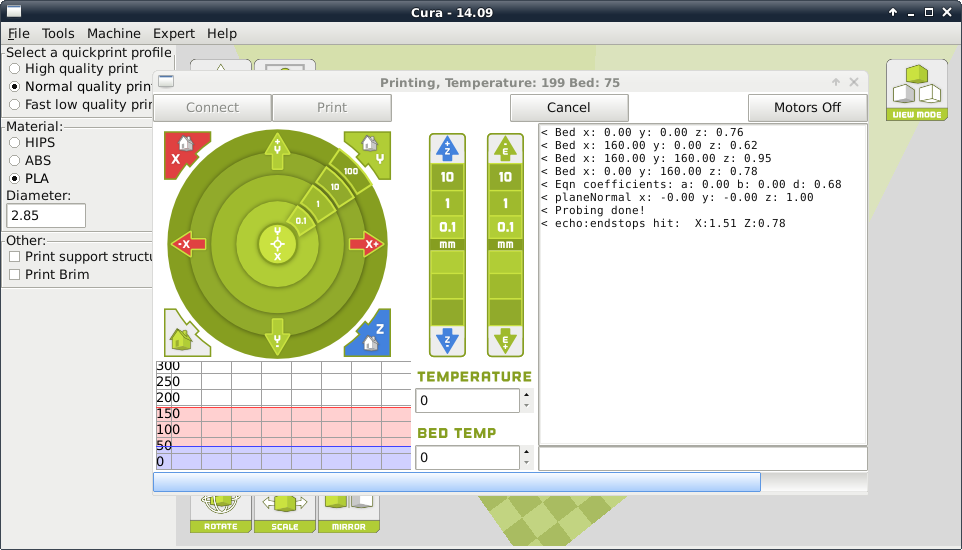
\includegraphics[keepaspectratio=true,angle=0,height=0.4\textheight,width=1.0\textwidth]{print_control.png}
%\caption{Print Control Screen}
%\label{fig:Print Control}
%\end{figure}

%\subsection{TAZ}

Your TAZ 3D printer has the ability to print directly from a computer using the included USB cable, or directly from the SD card by using the Graphical LCD controller.

%%%% SD Printing %%%%
\subsection{Printing from SD Card}
\index{Printing from SD}
\index{Graphical LCD controller}
\index{GLCD}
\index{SD card}
\index{SD}

Save your Gcode file to your SD card. Select \texttt{File} > \texttt{Save Gcode} and choose the SD card location. Insert the SD Card into the Graphical LCD Controller. 

\subsection{Set Temperature}

Turn on the heated bed and hot end by using the Graphical LCD controller and navigating to: \texttt{Temperature} > \texttt{Select Filament type}. If you are using other materials you can set your desired temperatures by going to \texttt{Temperature} > \texttt{Custom Temp} > \texttt{Nozzle/Bed}. Wait for your 3D printer to reach specified temperatures.

\subsection{Start Print}
\index{printing}
Once at the desired printing temperature begin your print through your Graphical LCD controller by navigating to: \texttt{Print From SD} > \texttt{Desired File}.

%%%% Tethered printing %%%%

\subsubsection{Printing from USB Cable}
\index{Printing from USB}

Connect your 3D printer to a computer using a USB cable, power it on and select the \texttt{Control} button at the top of the 3D viewing window. This will bring up your Pronterface user interface. You will not be able to send any commands until the window title changes to \texttt{Operational}. Once it is operational, you will need to set your filament specific temperatures. The temperature box heats the hot end, while the bed temp sets the bed temperature. Your current temperatures will be listed in the top of the control box. Once your hot end and bed are heated, select \texttt{Print}. This will start the printing process.

\begin{figure}[H]
\centering
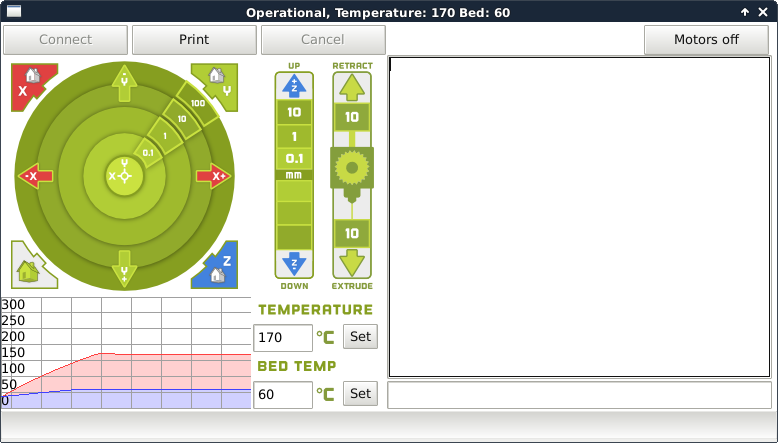
\includegraphics[keepaspectratio=true,angle=0,height=0.4\textheight,width=1.0\textwidth]{Pronterface117.png}
\caption{Control Screen}
\label{fig:Control}
\end{figure}

%\subsection{Pausing Mid-print}
%\index{Pause}
%You will notice after starting your print, the print button has changed to a pause button. This will pause your print after it has run through its Gcode buffer. Cura will remember the location of your print heads X and Y coordinates if moved through Cura. This allows you to move the print head away from your print and change filaments, colors, etc. When you hit resume, Cura will bring the print head back to the original (X,Y) before resuming. Disabling the motors, and manually moving the print head will cause Cura to lose the (X,Y) positioning. \textcolor{red}{Cura will NOT remember any Z movements}. If you would like to move in the Z direction, be sure to make the opposite movement before resuming.

\subsection{Recommended Temperatures}
\index{Temperatures}
When preparing your printer for operation, please be sure to set your temperatures, in Celsius, to the specific filament you are using. 
\begin{center}
 \hspace*{-1.5cm}\begin{tabular}{||c c c c c||} 
 \hline
 Filament Type & Bed Preparation & Nozzle Temp & Bed Temp & Removal Temp \\ [0.5ex] 
 \hline\hline
 ABS & Clean PEI & 240-260 & 110 & 50 \\ 
 \hline
 PLA & Clean PEI & 195-215 & 60 & 45 \\
 \hline
 HIPS & Clean PEI & 240-260 & 110 & 50\\
 \hline
 Laywoo-D3 & Clean PEI & 175-195 & 60 & 45 \\
 \hline
 Laybrick & Clean PEI & 175-195 & 60 & 45 \\
 \hline 
 Magnetic Iron PLA & Clean PEI & 220-230 & 60 & 45 \\
 \hline
 Stainless Steel PLA & Clean PEI & 220-230 & 60 & 45 \\
 \hline
 t-glase & Glue stick & 240-260 & 60 & 45 \\
 \hline
 Flexible Filaments & Glue stick & 215-230 & 50 & 35 \\  
 \hline
 Nylons & Glue stick & 220-270 & 110 & 50 \\
 \hline
 Polycarbonate & Glue stick & 260-300 & 110 & 50 \\ 
 \hline
 Polycarbonate + ABS & Glue stick & 260-280 & 110 & 50 \\
 \hline 
 Conductive PLA & Clean PEI & 215-230 & 60 & 50 \\
 \hline
 N-Vent & Glue stick & 220-260 & 110 & 50 \\ [1ex]
 \hline
 
\end{tabular}
\end{center}

%%mini:
%This will start the printing process: (set the appropriate temperatures, go through the auto-leveling procedure, and start printing your model).
%\pageref{fig:Print Control}).


\section{Removing Your First Print}
\index{Removing a Print}
After your first print has finished, you need to wait for the part to cool down.  Your parts will be easier to remove if you allow your heated bed to cool down to optimal temperature. This will allow the plastic to contract, making it easier to remove. 
%\texttt{Your print bed will move forward once it is ready to be removed.}

Once your heated bed has cooled, use the blue handled knife that was included with your toolkit to remove the item. Carefully insert the blade of the knife between your print and heated bed. Once underneath the part rotate the blade- lifting with the sharp edge into the part, to gently pop the piece off your plate.
%\begin{figure}[hbt]
%\centering
%\includegraphics[keepaspectratio=true,angle=0,height=0.4\textheight,width=1.0\textwidth]{remove_part.png} %%%% Photo needed %%%%
%\caption{Remove Part}
%\label{fig:Remove part}
%\end{figure}

\section{Full Settings}
\index{Full Settings}
\textcolor{red}{Full settings should not be used until enough experience with 3D printing has been gained to feel comfortable with all aspects of the printer and its operation. The Quickprint Mode will provide good results for most models.}
The first time Cura is launched it will default to the \texttt{Quick Print} interface. In order to have more control of your slicing and Gcode generation, switch to \texttt{Full Settings}. Select \texttt{Expert} > \texttt{Switch to full settings}. If a quickprint profile for your filament type is available, be sure to have it selected. This will automatically update the settings for that filament. The following tabs will now be available: Basic, Advanced, Plugins, and Start/End-Gcode. You will also have access to the Expert Settings. 
%\begin{figure}[H]
%\centering
%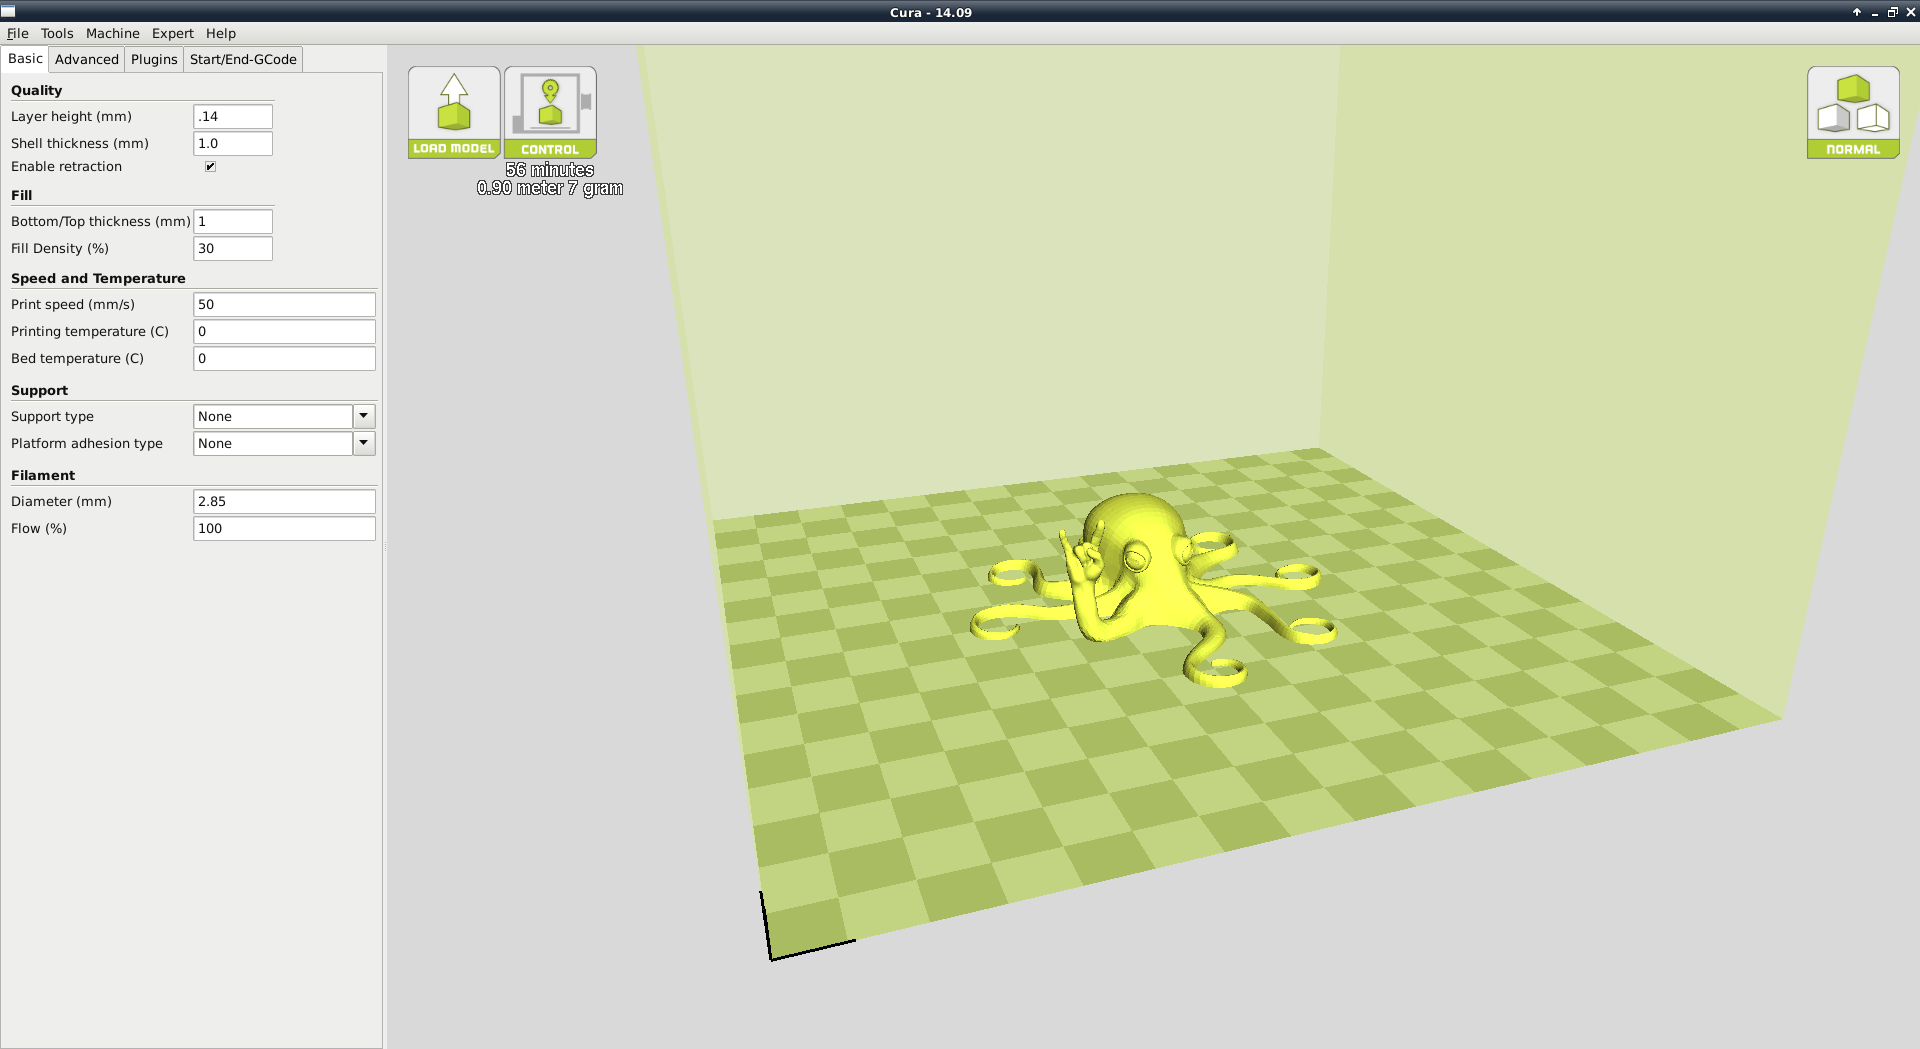
\includegraphics[keepaspectratio=true,angle=0,height=0.4\textheight,width=1.0\textwidth]{Expert.png}
%\caption{View in Full Settings}
%\label{fig:Full Settings View}
%\end{figure}
\begin{figure}[hbt]
\centering
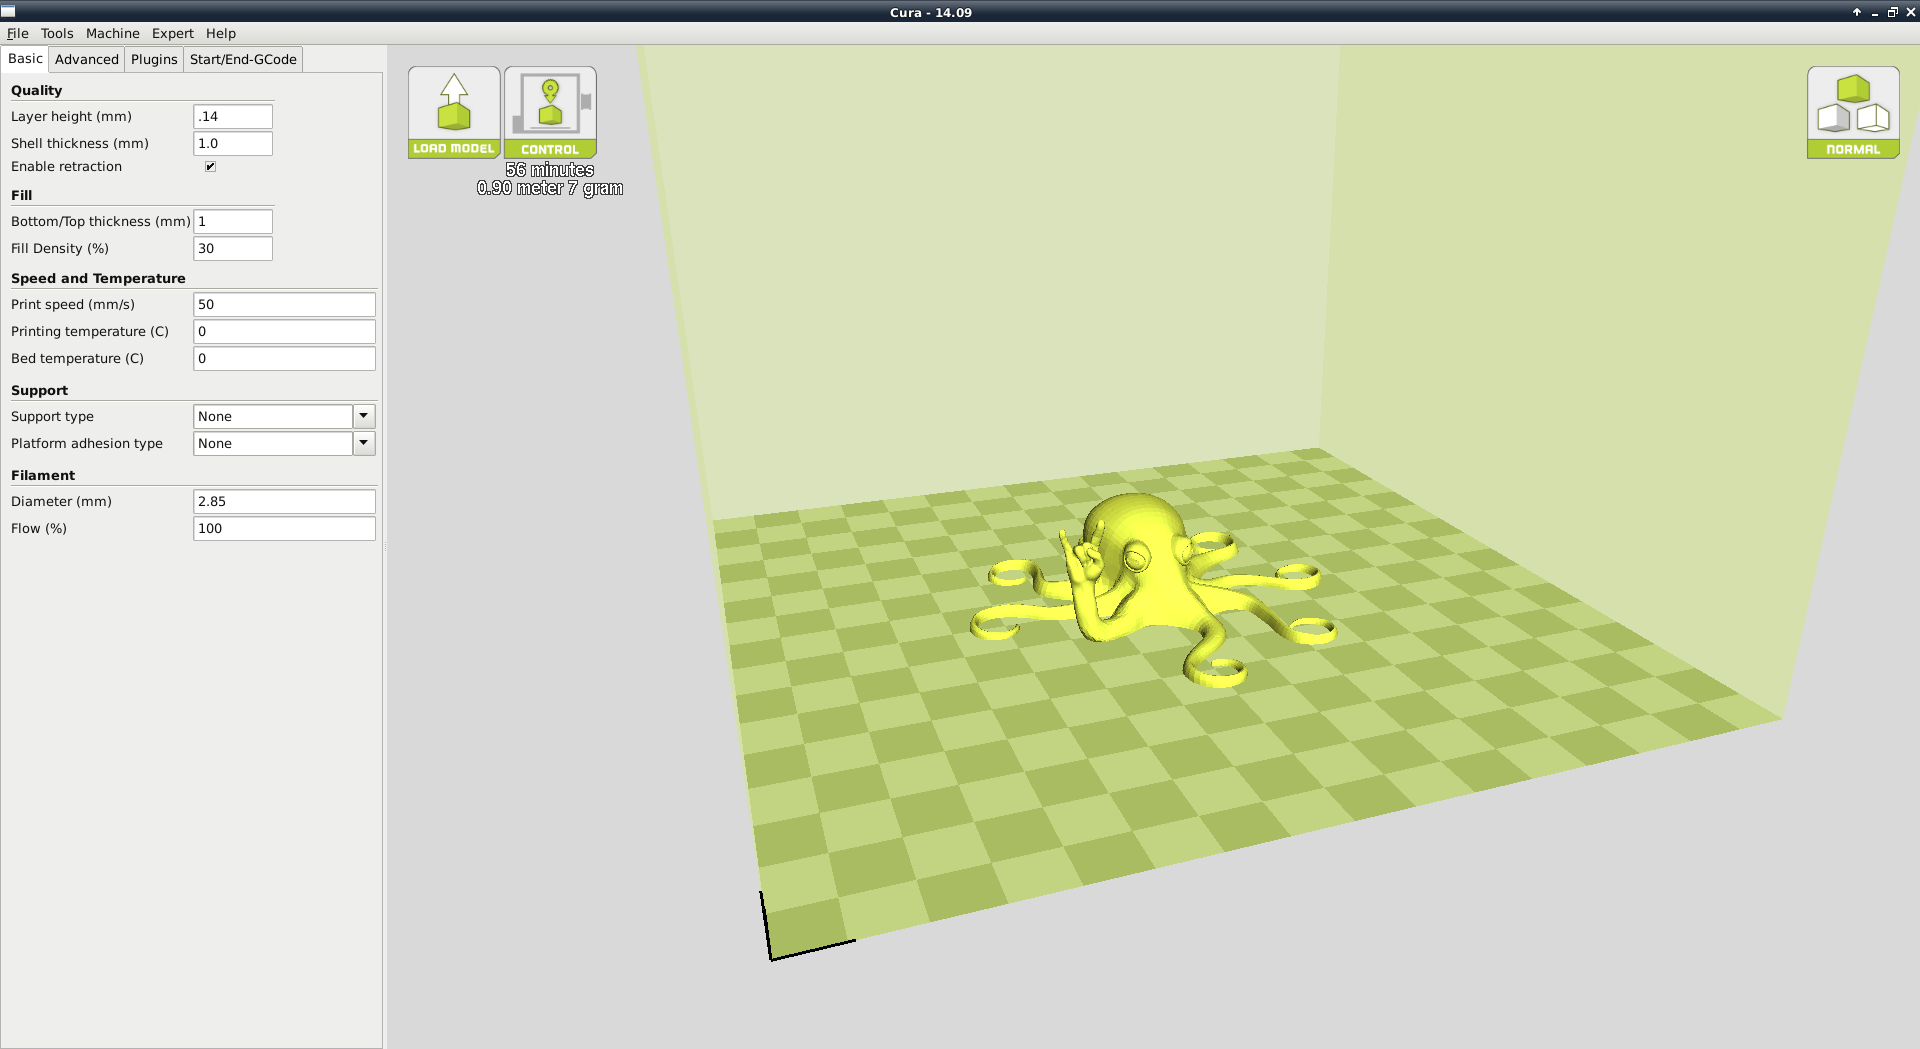
\includegraphics[keepaspectratio=true,angle=0,height=0.4\textheight,width=1.0\textwidth]{Expert.png}
\caption{Differences in Layer Height}
\label{fig:Differences in Layer Height}
\end{figure}
\subsection{View in Full Settings}
\index{Full Settings}
When you first switch to Full Settings, Cura will need to know what filament and quality you wish to use. It will automatically transfer our quickprint settings over to allow adjustments if one is selected. \textcolor{red}{IF A QUICKPRINT PROFILE IS NOT AVAILABLE, YOU WILL NEED TO MANUALLY LOAD ONE IN.} We recommend using our tested profiles that are available here: \texttt{https://www.lulzbot.com/support/downloads}. You will want to choose the profile that matches your filament and quality needs. Once downloaded, you can load the file into Cura by selecting \texttt{File} > \texttt{Open Profile}. Choose your desired profile. This will automatically update all of your settings for use with your printer.
%\begin{figure}[hbt]
%\centering
%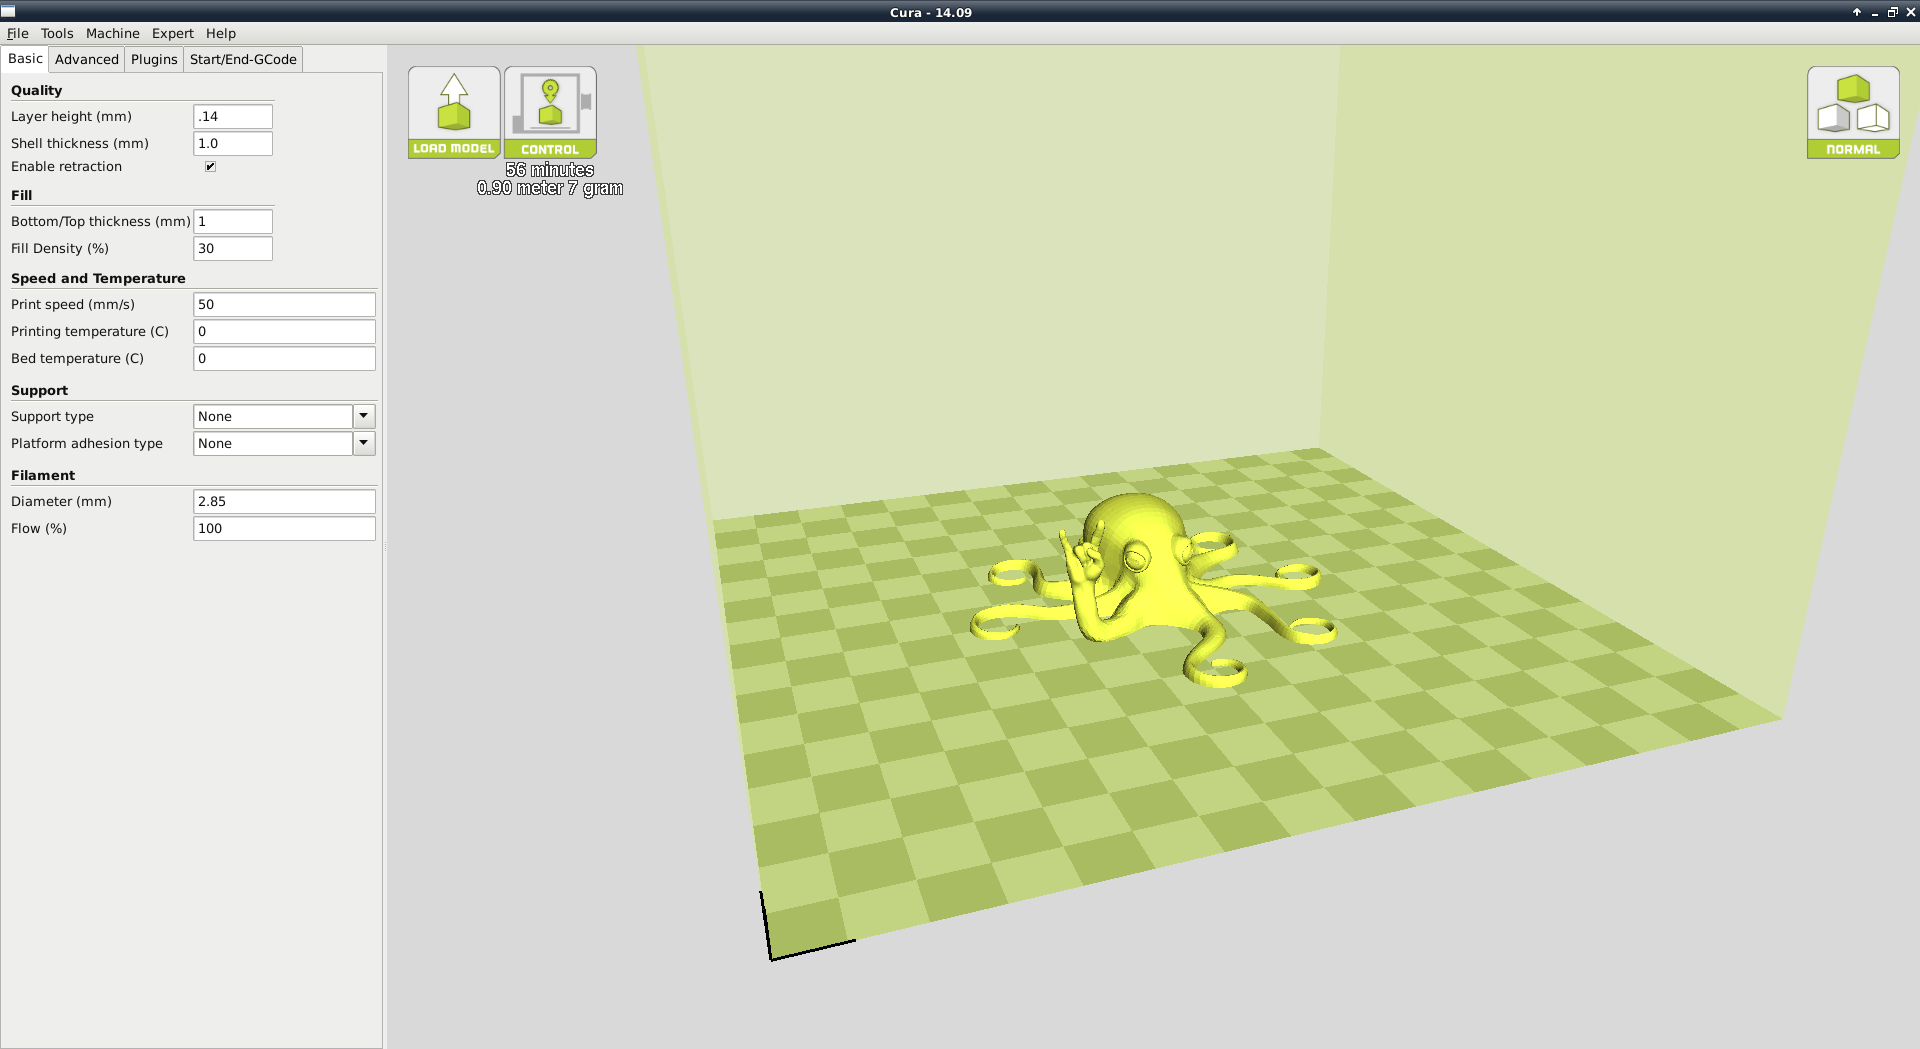
\includegraphics[keepaspectratio=true,angle=0,height=0.4\textheight,width=1.0\textwidth]{Expert.png}
%\caption{View in Full Settings}
%\label{fig:Full Settings View}
%\end{figure}

\section{Basic Tab Options}
\index{Basic Options}

\subsubsection{Layer Height}
\index{Layer Height}
The thickness of each printed layer is known as the \texttt{Layer Height}. The smaller the layer height, the smoother curves will appear. Larger layer heights are better for bridging and overhangs. Smaller layer heights will also increase print time, as it will take more layers to complete the object.
% (Layer height comparison photos)
\begin{figure}[H]
\centering
\includegraphics[keepaspectratio=true,angle=0,height=0.4\textheight,width=1.0\textwidth]{Layer_Height.jpg}
\caption{Differences in Layer Height}
\label{fig:Differences in Layer Height}
\end{figure}


\subsubsection{Shell Thickness}
\index{Shell Thickness}
This defines the number of vertical walls that comprise the outside of your model. We recommend keeping this set to multiples of your nozzle width. Your TAZ 3D printer is equipped with a 0.5mm nozzle. %The TAZ ships with a .5mm nozzle standard, while the Mini has a .5mm nozzle standard.

\subsubsection{Enable Retraction}
\index{Retraction}
Retraction tells your printer to pull filament out of the hot end upon travel moves. Travel moves are when your print head moves from one area of the print, to another without laying down filament. We recommend keeping this on for all filament types, and adjusting the retraction length and speed for the specific filament.
%(Details given in advanced tab section. ((Reference?))

\subsubsection{Bottom/Top Thickness (mm)}
\index{Bottom Thickness}
\index{Top Thickness}
Also known as \texttt{Surface Layers}- this will determine how thick the top and bottom layers are. A larger number here will create a thicker top and bottom which can be helpful for strength, bridging, and quality purposes. We recommend keeping this number as a multiple of your layer height.

\subsubsection{Fill Density}
\index{Fill Density}
This number is expressed as a percentage. 0\% will give a completely hollow print, while 100\% will give you a completely solid object. We have found that 20\% to 40\% fill density is functional for most prints.

\subsubsection{Perimeters Before Infill}
This option will toggle in what order the infill and perimeters are printed. We recommend leaving this toggled.
\subsubsection{Print Speed (mm/s)}
\index{Print Speed}
Your overall printing speed can be adjusted here. If no other speeds are determined in the later sections your printer will automatically default to this speed. This speed will be different, depending on what type of filament you are using.

\subsubsection{Printing Temperature}
\index{Printing Temperature}
%When using different filament materials you'll need to update the desired hot end and heated bed temperature. Any temperatures specified here will be used to automatically set both the hot end and heated bed. Your print will not begin until these temperatures are met. 

%The Mini 3D printer needs to have the temperature specified in order to run through the automatic bed-leveling routine.
%%%% Since the Mini needs to have Gcode temps set in order to run through auto bed leveling, the following statement is only applicable to the TAZ 4 or earlier. %%%%
We recommend leaving this temperature setting to “0”. If you set your temperature in this section your printer will not begin printing until it reaches the EXACT temperature. We recommend setting your printing temperatures through the Printer Interface, or through your LCD.

\subsubsection{Bed Temperature}
\index{Bed Temperature}
We recommend leaving this temperature setting to “0”. If you set your temperature in this section your printer will not begin printing until it reaches the EXACT temperature. We recommend setting your bed temperatures through the Printer Interface, or through your LCD.

\subsection{Support Type}
\index{Support Type}
Some models will require support material in order to print properly. This will usually occur when an object has an angle in relation to the build plate between 0 to 45 degrees. It is highly recommended to orient your object so that it minimizes or eliminates the need for support.

\subsubsection{Touching Buildplate}
This causes the support material to build up between the heated bed and the object. The red example is Touching Buildplate.
% (Photo of Circle inside a square, that is printed vertically. Have samples on photo table. Reference photo below?)

\subsubsection{Everywhere}
This prints support material between the heated bed and object as well as between the object and itself. The green example is Support Everywhere.
% (Photo of Circle inside a square, that is printed vertically, sample on photo table. Reference Photo Below?)
% (Support Comparison Photo)
\begin{figure}[H]
\centering
\includegraphics[keepaspectratio=true,angle=0,height=0.3\textheight,width=1.0\textwidth]{Support_Revised.png}
\caption{Support Types}
\label{fig:Different Types of Support}
\end{figure}

\subsection{Platform Adhesion Type}
\index{Adhesion Type}
Some models have a small surface area contacting the plate. This can create adhesion issues causing your part to pop off at some point during the print. To fix this, use either \texttt{Brim} or \texttt{Raft}. Raft is better used when a model has small heated bed contact points and overhangs.

\subsubsection{Brim}
\index{Brim}
Brim will create a single layer of filament, contacting and surrounding your model. This will increase the surface area of the part contacting the build platform thereby preventing it from popping off the heated bed. Brim will also help in situations where you are seeing corner lift. Brim settings can be adjusted in the \texttt{Expert Settings} options.
% (See Expert Settings/Page REFERENCE)

\subsubsection{Raft}
\index{Raft}
%% Raft is rarely used these days %%
Raft will generate a layer of material underneath your object. Raft was more often used before the addition of heated plates to increase surface area. Raft settings can be adjusted in the \texttt{Expert Settings} options.

\subsection{Filament Diameter}
\index{Filament Diameter}
The filament diameter setting is one of the more important settings. Make sure that you update this value periodically with your average filament diameter. While your filament may be referred to as 3mm, it is more likely going to be near 2.9mm +/- 0.1mm. You will want this to be an accurate average, as it will allow your printer to correctly calculate how much filament it is pulling into the hot end.

\subsection{Filament Flow \%}
\index{Flow Rate}
This controls how much filament your printer is extruding in relation to speed. This setting is mainly used to adjust for filament density variations. Leave this value at 100\% as changing it can lead to surface quality issues.

\section{Advanced Tab Options}
\index{Advanced Options}

\subsection{Nozzle Size (mm)}
\index{Nozzle Size}
%%%% standalone version line %%%%
This defines your nozzle size. The slicing engine uses this value combined with your other settings to determine how quickly to feed filament into your hot end. The TAZ ships with a 0.5mm nozzle. 

%This defines your nozzle size. The slicing engine uses this value combined with your other settings to determine how quickly to feed filament into your hot end. The Mini ships with a 0.5mm nozzle.

\subsection{Retraction Speed (mm/s)}
\index{Retraction Speed}
Retraction Speed determines the speed at which your filament is reversed out of the hot end for travel moves and when changing direction during printing. We recommend keeping this set to 25mm/s.

\subsection{Retraction Distance}
\index{Retraction Distance}
Retraction Distance determines how much filament is pulled out of your hot end on travel moves and when changing direction. You will want to adjust this depending on temperature settings and filament type. Higher thermal retaining filaments such as PLA behave better with a longer retraction distance. We have found anywhere from 1mm to 3mm is a good starting range.
% changed from "1 to 6mm" to remain conservative.

\subsection{Initial Layer Thickness}
\index{Initial Layer}
This will control how thick your first printed layer height is printed onto the heated bed. Having a larger initial layer height will help prevent your part from popping off the plate. All of our standard profiles have a 0.3mm initial layer height. This eliminates the need for adjustments when switching between filaments.  %\textcolor{red}{Your LulzBot\textsuperscript{\miniscule{\texttrademark}} Mini auto leveling system could be affected if you change this from the standard profiles. Adjust at your own risk.}
\subsection{Initial Layer Line Width}
\index{Initial Layer Width}
This will control how wide your first extruded filament path is for the initial layer. A wider line width will help with bed adhesion. We have found 125\% to be a good starting place. For models with moving printed in place parts, a smaller initial layer line width is recommended. %\textcolor{red}{Your LulzBot Mini auto leveling system could be affected if you change this from the standard profiles. Adjust at your own risk.}

\subsection{Cut Off Object Bottom (mm)}
\index{Cut Off Object}
This setting is used to help print models that were not specifically designed for FFF printing. In particular, it is for models that do not have a flat surface to adhere to the plate. It will sink your object Xmm into the build plate, creating a nice flat surface to begin your print. You can also use this option to remove the lower portion of your model, or if carefully measured, cut your part in half for printing object as two halves.
\begin{figure}[H]
\centering
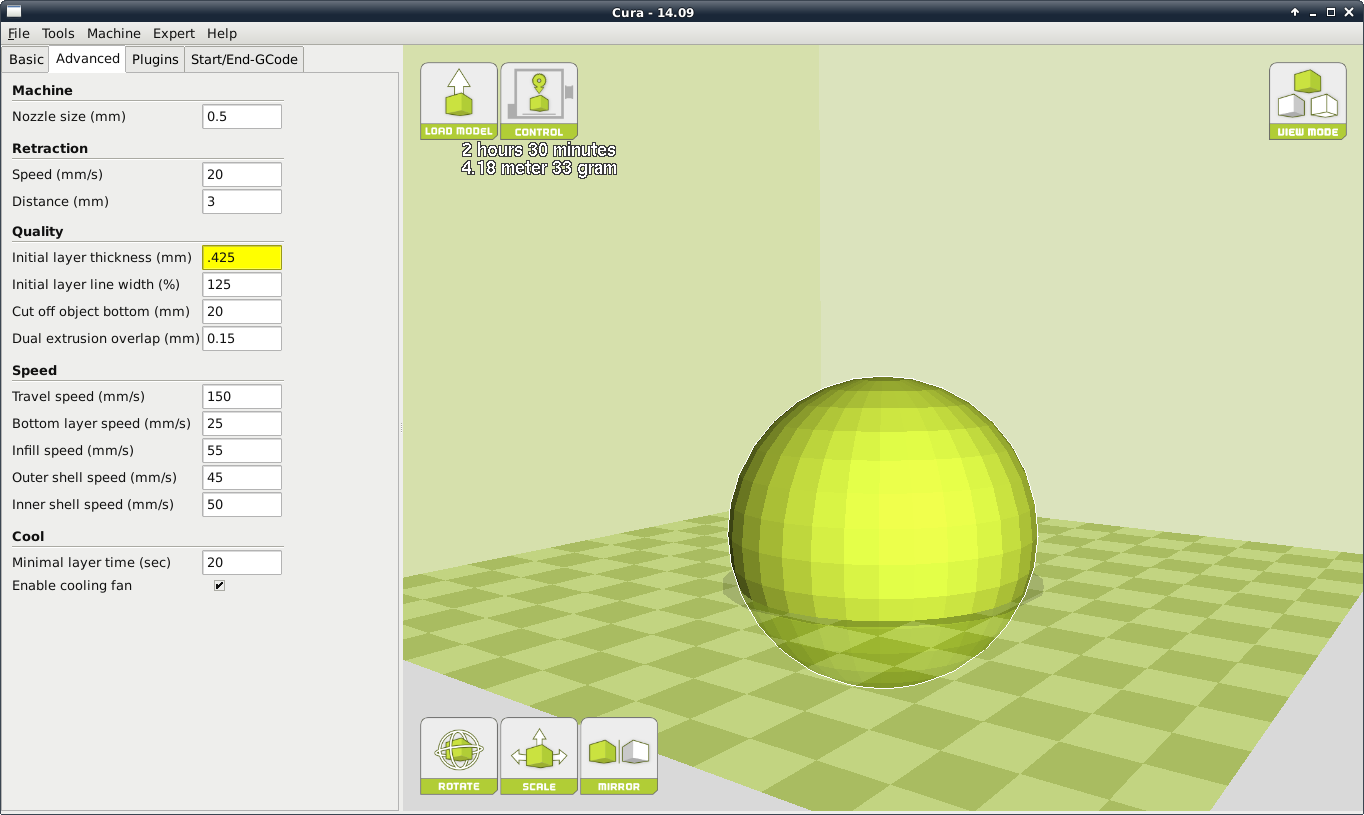
\includegraphics[keepaspectratio=true,angle=0,height=0.4\textheight,width=1.0\textwidth]{cutoff.png}
\caption{Cutoff Example}
\label{fig:Cutoff Example}
\end{figure}

\subsection{Dual Extrusion Overlap}
\index{Dual Extrusion Overlap}
This will determine how far your Dual Extruders will overlap when laying down material. This will help adhesion between the two different colors or types of filament. This setting is only used when the printer is equipped with two hot ends and extruders.

\subsection{Travel Speed}
\index{Travel Speed}
This setting will determine how fast your print head moves while not extruding filament. A normal travel speed of 125 - 175mm/s is recommended.

\subsection{Bottom Layer Speed}
\index{Bottom Layer Speed}
This will control your initial layer speed. In general, a slower initial layer speed will help with first layer adhesion. 

\subsection{Infill Speed}
\index{Infill Speed}
This is how fast your print head speed will be while laying down the interior portion of your model. Faster speeds are usually tolerable here, as none of the infill will be visible from the outside of your object. If you go too fast compared to your inner and outer shells, you can have adhesion issues or globs of filament left behind from the print head.

\subsection{Outer Shell Speed}
\index{Outer Shell Speed}
This will be the outermost surface of the model. This is the most important speed setting, as it controls the speed of your print head on the visible layers. As a general rule of thumb, the slower you go the better looking print you will get. 

\subsection{Inner Shell Speed}
\index{Inner Shell Speed}
This affects vertical walls that are in between the outer shell and infill. This will not be visible but will help support the outer shell and the infill. We recommend keeping this speed setting between your infill and your outer shell speed.

\subsection{Minimal Layer Time}
\index{Minimal Layer Time}
This will determine a minimum amount of time your printer will spend laying down each layer. If your layer print time falls below this your printer will automatically slow down to reach this time before moving onto the next layer. Tweaking this can help get cleaner, crisper prints.

\subsection{Enable Cooling Fan}
\index{Enabling Cooling Fan}
Enables operation of your extruder active cooling fan. The fan settings can be adjusted in the \texttt{Expert Settings} options.

\section{Plugins}
\index{Plugins}
Plugins are custom settings which will alter your print at specific points. The two that come preloaded with Cura are \texttt{Tweak at Z}, and \texttt{Pause at Height}. More plugins and information can be found here: \texttt{http://wiki.ultimaker.com/Category:CuraPlugin} To activate one of these highlight the desired plugin and click the drop-down arrow directly below the Plugins box. 
\begin{figure}[H]
\centering
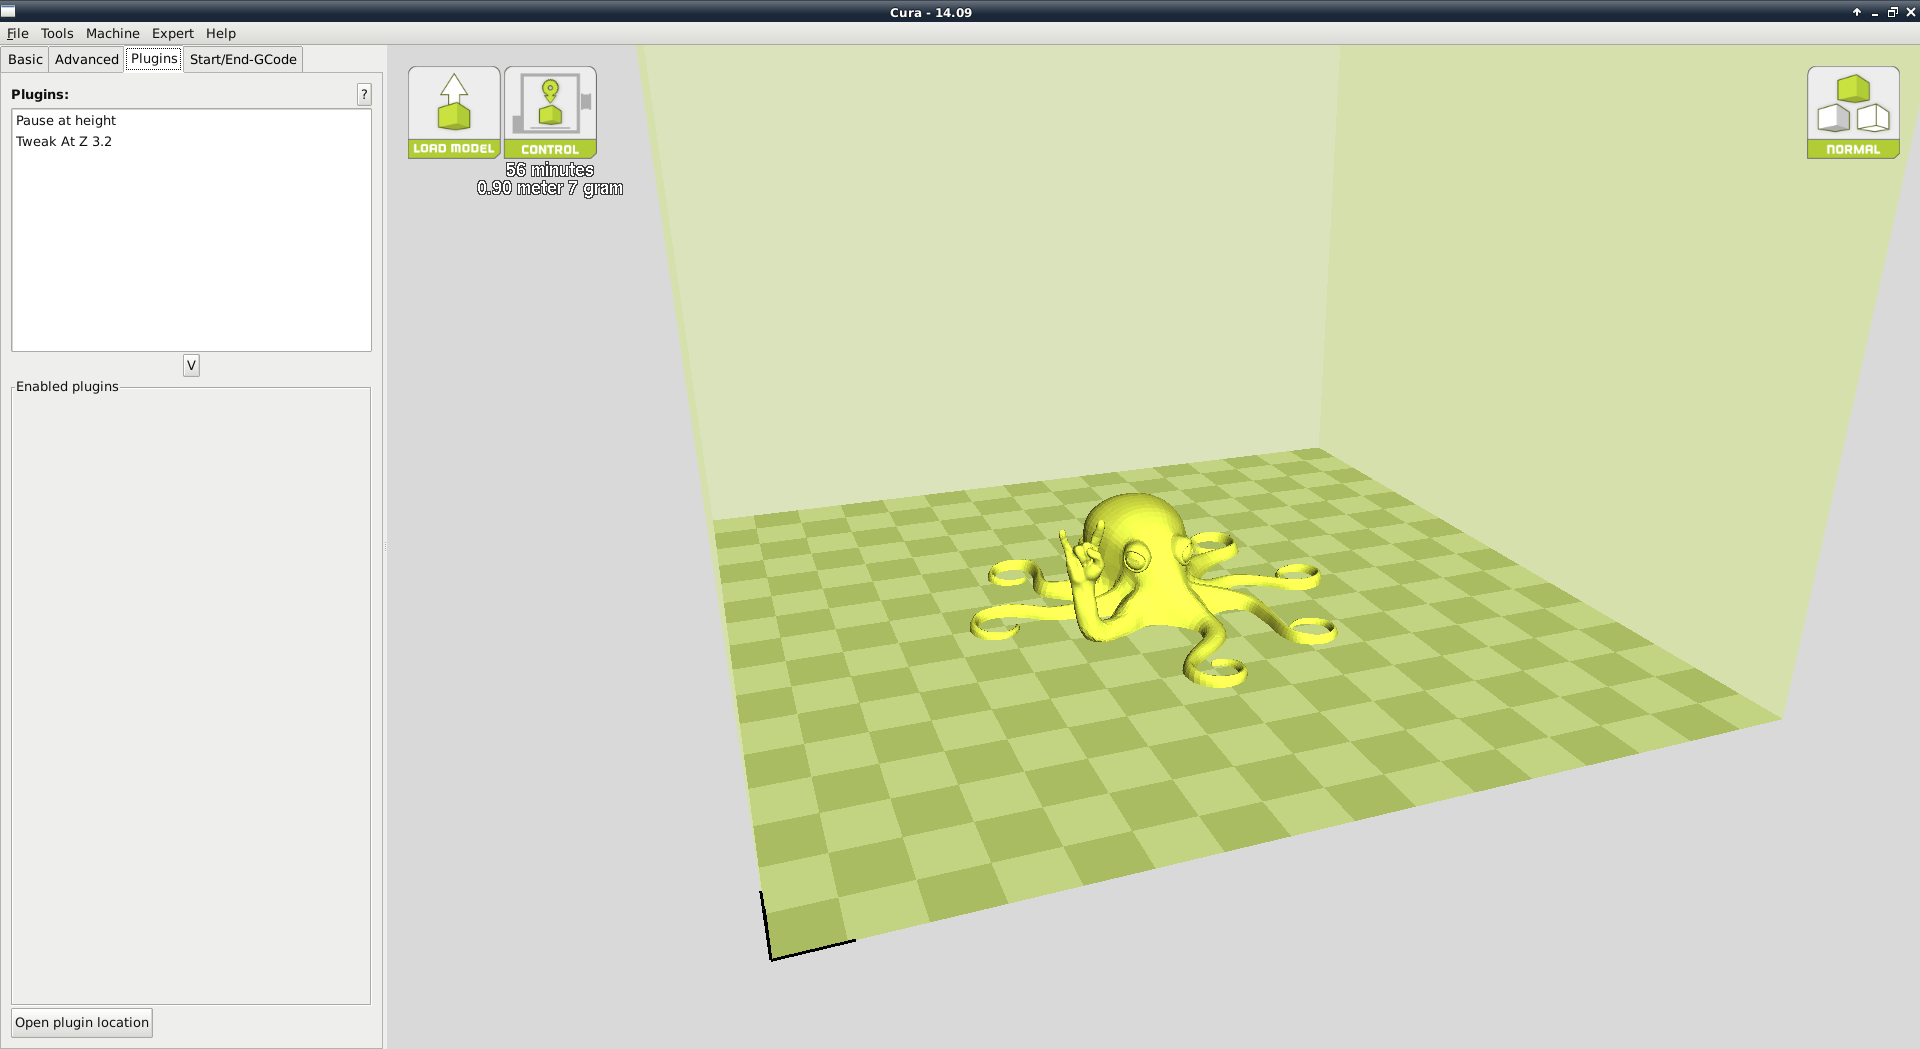
\includegraphics[keepaspectratio=true,angle=0,height=0.4\textheight,width=1.0\textwidth]{Plugins.png}
\caption{View of Plugins}
\label{fig:Plugins}
\end{figure}

\subsection{Tweak at Z}
\index{Tweak at Z}
Make basic changes at specified Z heights. You can determine the Z height or layer count at which you want to make a change. Then choose how you would like to change your settings. You can alter temperatures, fan speeds, and print speeds. Fine tuning these for specific STL files, can produce cleaner prints.

\subsection{Pause at Z Height}
\index{Pause at Z Height}
Pause your print at a specified height. You can also specify where to move the print head and how much filament to retract. This will prevent “blobs” from accumulating on your print while paused. This setting is most commonly used when switching colors of filaments in the middle of a print.

\section{Start and End Gcode Settings}
\index{Custom Gcode}
Custom Gcode allows for complex automatic printer movements and operations. By adding custom Gcode into the start or end of your file, you can alter how it prints. A comprehensive list of Gcode commands can be found here: \texttt{http://reprap.org/wiki/G-code} We recommend new users to leave this as provided in the profiles at \texttt{https://www.lulzbot.com/support/downloads}

%mini
%\subsection{Mini Specific Considerations}
%Please be cautious when changing any of these start and end Gcode settings. \textcolor{red}{This is where your Auto Bed Leveling commands are stored. If improperly altered, your printer will no longer automatically compensate for the heated bed position and can even potentially damage components on the printer.} If you are uncertain of the change you are trying to make, please contact us at \texttt{Support@LulzBot.com} before hand.

\section{Expert Settings}
\index{Expert Settings}
Expert settings will give you more specific options for your retraction, skirt, active cooling, infill, support, brim, raft, and special settings. To gain access to this section you go to \texttt{Expert} > \texttt{Open Full Settings} or on your keyboard press \texttt{Control + E}.
\begin{figure}[H]
\centering
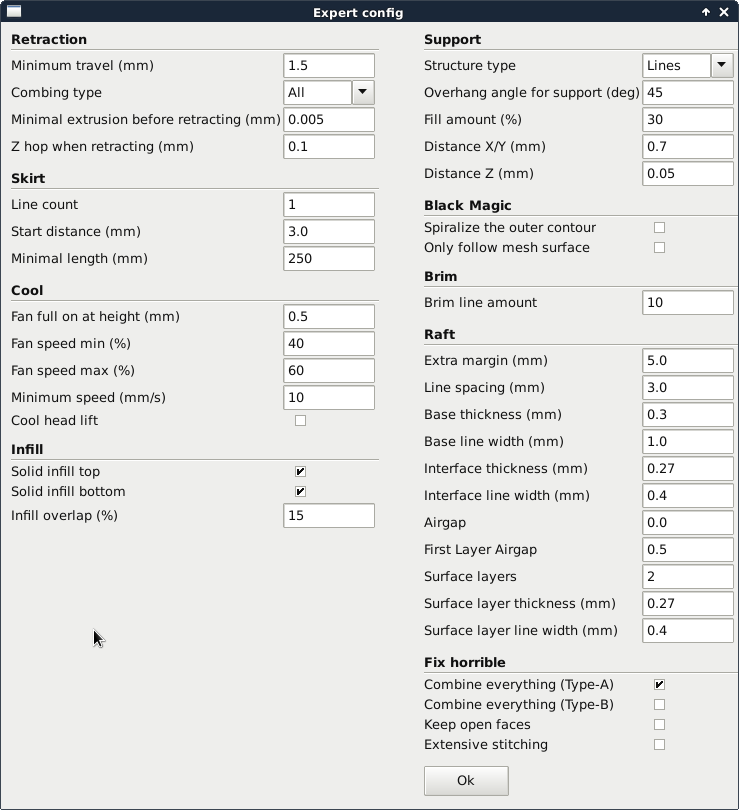
\includegraphics[keepaspectratio=true,angle=0,height=0.4\textheight,width=1.0\textwidth]{Expert_Settings.png}
\caption{View Expert Settings}
\label{fig:Expert Settings}
\end{figure}

\section{Retraction}
\index{Retraction}
Retraction pulls filament out of your nozzle when it is not extruding to prevent your print head from dripping on your object. This section is where you will control how your extruder retracts its filament.

\subsection{Minimum Travel}
\index{Minimum Travel}
This sets the minimum travel distance of your print head in order to retract. If your print head is not moving this far during travel moves, it will not retract.

\subsection{Combing}
\index{Combing}
This option prevents your print head from traveling over holes in the X/Y plane when printing. This will slightly increase print time, but will prevent strings from getting caught on the holes during travel moves. We recommend keeping this setting on.

\subsection{Minimal Extrusion Before Retracting}
This will prevent a retraction move, if your extruder has not put out Xmm of filament since its last retraction.

\subsection{Z Hop When Retracting}
\index{Z hop}
This will raise your print head Xmm while retracting. This setting helps prevent ooze, and strings from being deposited on your print. 
%\textcolor{red}{We do not recommend this setting for TAZ 3 users and earlier. This can cause issues with Z dimensional accuracy.}

\section{Skirt}
\index{Skirt}
Skirt creates a line around the outside of your object. Most commonly used to prime the extruder, in order to prevent missed filament at the beginning of a print. Leave this setting on.

\subsection{Line Count}
\index{Line Count}
This will define the number of loops the Skirt creates around the outside of your object. Smaller models will require more loops to properly prime the extruder.

\subsection{Start Distance}
\index{Start Distance}
This will define the distance away from your model that the skirt will be created. 

\subsection{Minimal Length}
\index{Minimal Length}
This will define the minimum extruded line length for the skirt. This will over ride your line count, producing as many lines as required to reach the minimal length.

\section{Cool}
\index{Cooling}
This section will define how your extruder cooling fan will operate during the print. \textcolor{red}{Your fan will not start until it has reached 25\% or higher for speed settings.} If your print speeds are slowed down due to minimal layer time, the fan will run between minimum and maximum speed based upon how much the layer is slowed down.

\subsection{Fan on at Full Height}
\index{Fan Settings}
This is your Z height where your fan will be turned on to its minimum percentage setting. Especially helpful with high temperature retaining filaments such as PLA. This will be scaled between 0\%, and your minimum fan speed based upon layer height; with it being disabled for the first layer.

\subsection{Fan Speed Min}
\index{Fan Settings}

This will be the speed your fan runs when enabled at full height. Once the Z height is reached for Fan on at Full Height, this will be the speed your fan runs at.

\subsection{Fan Speed Max}
\index{Fan Settings}
This is the fastest speed at which your fan will ever run. When your print speed is slowed down due to minimal layer time, your fan will run between minimum and maximum speed. The maximum fan speed is reached when your printer must be slowed by 50\% or greater.

\section{Support}
\index{Support Material}
You define how your support material is generated here. You must have some form of support turned on in the basic settings in order for these settings to have an effect.

\subsection{Structure Type}
\index{Support Settings}
You can choose between a Grid or a Line pattern for your support material. The grid will be a checkerboard pattern in the X and Y direction. The line option will produce lines in along the y axis for support. The grid will provide stronger support than the line option, but will be harder to remove.

\subsection{Overhang Angle for Support}
\index{Overhang Angle}
This will determine where support material is generated. In general you will be able to print a model with 45 to 90 degree angles in relation to the bed without support. We recommend leaving this setting at 45 degrees.

\subsection{Fill Amount}
\index{Fill Amount}
This will determine how dense your support material is printed, similar to Infill Percentage. The higher percentage, the better support, but it will be harder to remove the support material, will use more material, and will lead to a larger total printing time.

\subsection{Distance X/Y}
\index{Support}
This will determine how far away from your object in the X/Y plane that the support material is being placed.

\subsection{Distance Z}
\index{Support}
This will determine how far away your support material is from your object in the vertical direction. A smaller number here makes for better support, but makes it harder to remove.

\section{Black Magic}
\index{Black Magic}
This section allows you to transform your model into a hollow shell, a single layer thick.

\subsection{Spiralize the Outer Contour}
\index{Spiralize}
This causes your Z axis to be constantly moving upward as printing your single outer wall shell. The results are no layer change lines, giving a much smoother surface. This setting is typically only used for artistic objects as they will be fragile.

\subsection{Only Follow Mesh Surface}
\index{Black Magic}
This will cause your print to follow the outside of your model, building it completely hollow with a single wall outer shell. The only difference between this and Spiralize, is that the Z axis moves regularly. That is, it prints a layer and then moves up to the next one.

\section{Brim}
\index{Brim}
Brim circles the base of the print while making contact, helping adhere the print to the heated plate. This is only one layer thick, and easily removed post-print. This section defines how the brim is formed when brim is activated in basic settings.

\subsection{Brim Line Amount}
This will determine the distance the brim will cover around the outside of your object. The more brim used, the better your part will adhere to the plate. 

\section{Raft}
\index{Raft}
Raft is a platform built underneath your object, designed to help adhesion and prevent warping. It will lay down support material, and then a platform on top of the supports. Your model will be built on top of this platform. The bottom surface of your printed part will not be as clean or as even when using this option. Raft is typically not required.

\subsection{Extra Margin}
\index{Extra Margin}
This determines the distance around the outside of your object that the raft is created. Can be helpful for ensuring no warping of the lower layers.

\subsection{Line Spacing}
\index{Line Spacing}
This will determine the spacing between “support” lines for the raft. A small spacing makes the support structures closer together improving strength of the raft, but uses more material.

\subsection{Base Thickness}
\index{Base Thickness}
This defines how thick your raft will be.

\subsection{Base Line Width}
\index{Base Line Width}
This will define how wide your “support” material is for the raft. This setting will determine how well the surface layers of the raft print.

\subsection{Interface Thickness}
\index{Interface Thickness}
This will determine how thick the surface layers of the raft are. The surface layers are the platform that is built upon the supports.

\subsection{Interface Line Width}
\index{Interface Line Width}
This will determine how wide the top layers of the platform will be. In general, you can keep this set to your nozzle size, as surface quality of the removable raft is not important.

\subsection{Airgap}
\index{Airgap}
This will define the distance between your raft and your print. A larger gap will make your part easier to remove, but will make the bottom of your print look worse.

\subsection{Surface Layers}
\index{Surface Layers}
This will determine the number of layers that create the “platform” of your raft. If you have a wide line spacing, you may want to increase this number to ensure a solid platform. 

\section{Fix Horrible}
\index{Fix Horrible}
These are some of the more advanced and experimental options. They are designed to help repair models with errors to make them suitable for 3D printing. They do not always work. Please be cautious when using these options as they can have unintended effects on your print quality.

\subsection{Combine Everything (Type-A)}
\index{Combine Type-A}
This will attempt to fix all external mesh errors, while keeping internal holes intact. This can accidentally fill in intentional internal holes.

\subsection{Combine Everything (Type-B)}
\index{Combine Type-B}
This will ignore all internal holes of the model and only focus on the external holes. This is helpful when only the outside finish of the model is important.

\subsection{Keep Open Faces}
\index{Open Faces}
This will ignore all manifold errors in the object. It can create issues generating the Gcode as Cura does not know how to interpret the open holes. This option should only be used if you are sure that the holes in the mesh are intended. In general, you should not use this option.

\subsection{Extensive Stitching}
\index{Extensive Stitching}
This causes Cura to automatically add triangle meshes in an attempt to fix manifold errors. This algorithm will greatly increase Gcode generation time and may end up adding in un-intended meshes. It is recommended that you repair your model through MeshLab, FreeCAD or your preferred CAD program before attempting this option.

\section{Dual Extrusion}
\index{Dual Extrusion}
The LulzBot TAZ has the ability to add dual extrusion functionality with the Dual Extruder tool head add-on. We only recommend the Dual Extruder tool head for advanced users. Installation and operation of the dual extruder will require you to flash your firmware, calibrate your extruders, level two heads to a single plane, define extruder offsets, and fine tune your slicing profile. This can be a little overwhelming for new users. We recommended that you have a couple of months of single extruder printing experience before making the switch.

\subsection{Updating Firmware}
\index{Updating Firmware}
In order to use the Dual Extruder you will need to update your firmware to activate the second hot end.

\begin{itemize}
\item Power on your 3D printer and connect it to your computer through USB.
\item Select \texttt{Machine > Add New Machine}.
\item The next window that opens will display several different LulzBot 3D printers. Select your model, the \texttt{TAZ 5}.
\item Choose the correct hot end and select \texttt{Next}.
\item Select the appropriate tool head for your TAZ and select \texttt{Next}.
\item Choose the correct nozzle size for your machine. If you are not sure what size your printer has use your serial number to determine the nozzle size with the information found at \texttt{https://www.lulzbot.com/printer-identification}.
\item The final step will be a firmware update. Choose \texttt{Flash the firmware} to continue with the update.
\item Once the progress bar has completed select \texttt{OK > Next > Finish}.  
\item You can verify this by looking at the LCD screen. You should now see three temperature readings. 
\end{itemize} 
You can revert the firmware back to the stock configuration for your LulzBot\textsuperscript{\miniscule{\texttrademark}} 3D printer by selecting \texttt{Machine > Install default firmware}. Doing so will overwrite any of your current firmware settings.

\subsection{Preparing Cura}
In order to slice for a second tool head, you will need to let Cura know that you have added a second tool head. 
\begin{itemize} 
\item Select \texttt{Machine > Machine Settings > Extruder Count > 2}.
\item Select \texttt{Ok} to close out the screen.
\item Select \texttt{Machine > Machine Settings} to open the Machine settings again. 
\item A new section labeled \texttt{Extruder 2} is now present. Within it you will see an \texttt{X offset and Y offset}.
\item Set the \texttt{X offset to 0} and the \texttt{Y offset to -50}.
\item Select \texttt{Ok} to save your changes. The Machine settings window will close.
\end{itemize} 


\subsection{Calibrating Extruders}
\index{Calibrating Extruders}
Each individual extruder will have its own unique set of Esteps. To determine this, you will need to tell the extruder to take in 100mm of filament.
\begin{itemize}
\item Load the outer and inner calibrations squares into Cura \texttt{https://www.lulzbot.com/support/downloads}
\item Open the Printer Interface window and set temperatures for both heads. Switch between hot ends by entering ``\texttt{T0}'' for the rear extruder into the command line terminal. Press \texttt{enter}.
\item Type ``\texttt{T1}'' for the front extruder into the command line terminal. Press \texttt{enter}.
\item Make two marks at 100mm and 120mm on the filament from the top surface of each extruder.
\item Once at the correct extrusion temperature type into the command line ``\texttt{G92}'' and press \texttt{enter}. Then ``\texttt{G1 E100 F60}'' and press \texttt{enter}.
\item Switch to the other tool head by entering ``\texttt{T0}'' for the rear or ``\texttt{T1}'' for the front. 
\item Type into the command line ``\texttt{G92}'' and press \texttt{enter}.
\item Type ``\texttt{G1 E100 F60}'' and press \texttt{enter}.
\item Measure the distance that the tool head over or under extruded. You will need to adjust your Esteps by 8 up or down for each mm it under or over extruded.
\item Update your Esteps for the rear extruder and E1steps for the front extruder through your LCD screen. \texttt{Configuration > Advanced Settings > E/E1 Steps > New Number}. Push in on the knob to exit out of the Esteps entry.
\item Store your new Esteps \texttt{Configuration > Store Memory}.
\end{itemize}

\subsection{Defining Second Extruder Offset}
\index{Second Extruder Offset}
To get crisper looking prints, you will want to really dial in your offsets. With the outer and inner square on your build platform, right click and select \texttt{Dual Extrusion Merge}. The red square will be printed with your front extruder, and the yellow square will be printed with the rear extruder.
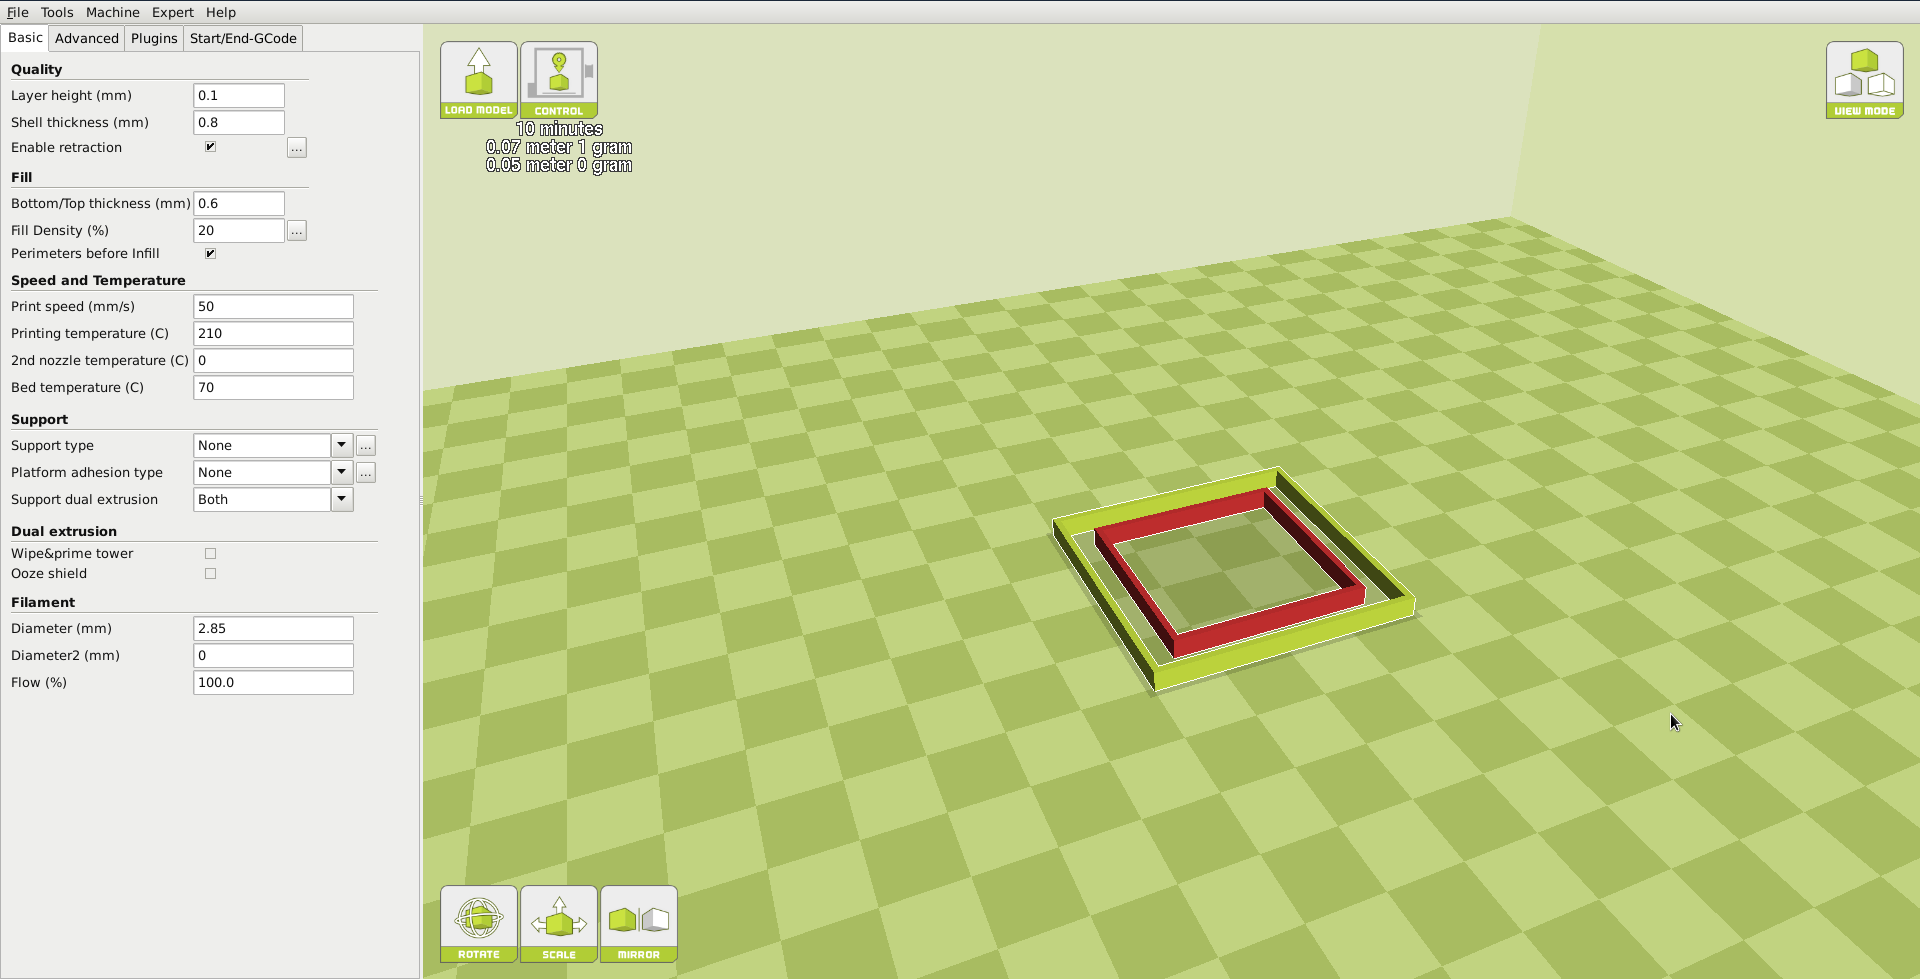
\includegraphics[keepaspectratio=true,angle=0,height=0.4\textheight,width=1.0\textwidth]{CalSquares1.png}
After printing the squares, you will want to measure Top, Bottom, Left, and Right gap. Enter these numbers into our offset calculator found here: \texttt{https://www.lulzbot.com/dual-extruder-calibration-calculator} This will produce new offsets, that will need to be updated in the Machine Settings menu. Repeat as many times as desired to truly fine tune the offset. 

\subsection{First Dual Print}
\index{First Dual Print}
When you are ready to produce your first dual extrusion print, you will need to combine the two separate STL files. One STL file will be for each print head. \texttt{Left Click} on whichever STL you would like printed with the \texttt{Rear Tool head}. Then \texttt{Right Click} on whichever STL file you would like printed with the \texttt{Front Tool head} and select dual extrusion merge. You will now see a single model in two colors on the build plate. The red section will be printed with the fron extruder, while the green section will be printed with the rear extruder. 
\begin{figure}[H]
\centering
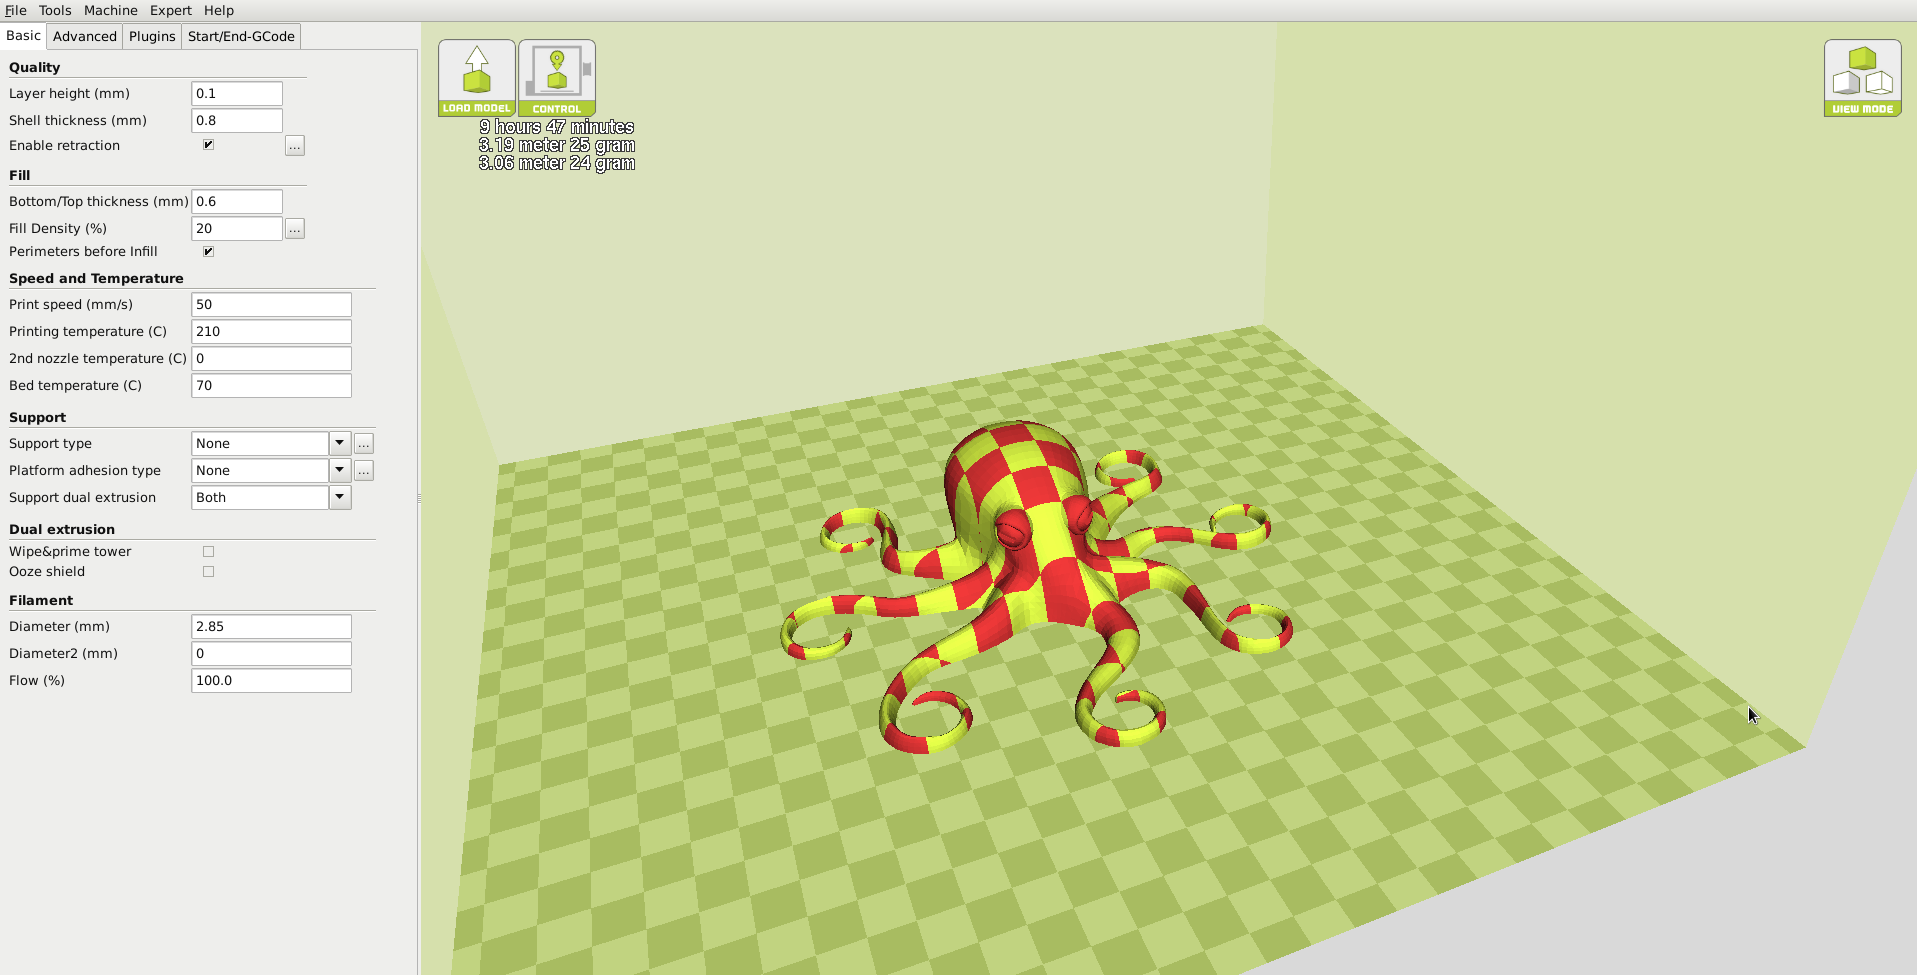
\includegraphics[keepaspectratio=true,angle=0,height=0.4\textheight,width=1.0\textwidth]{PostMerge.png}
\caption{After Merge}
\label{fig:After Merge}
\end{figure}

\begin{figure}
\centering
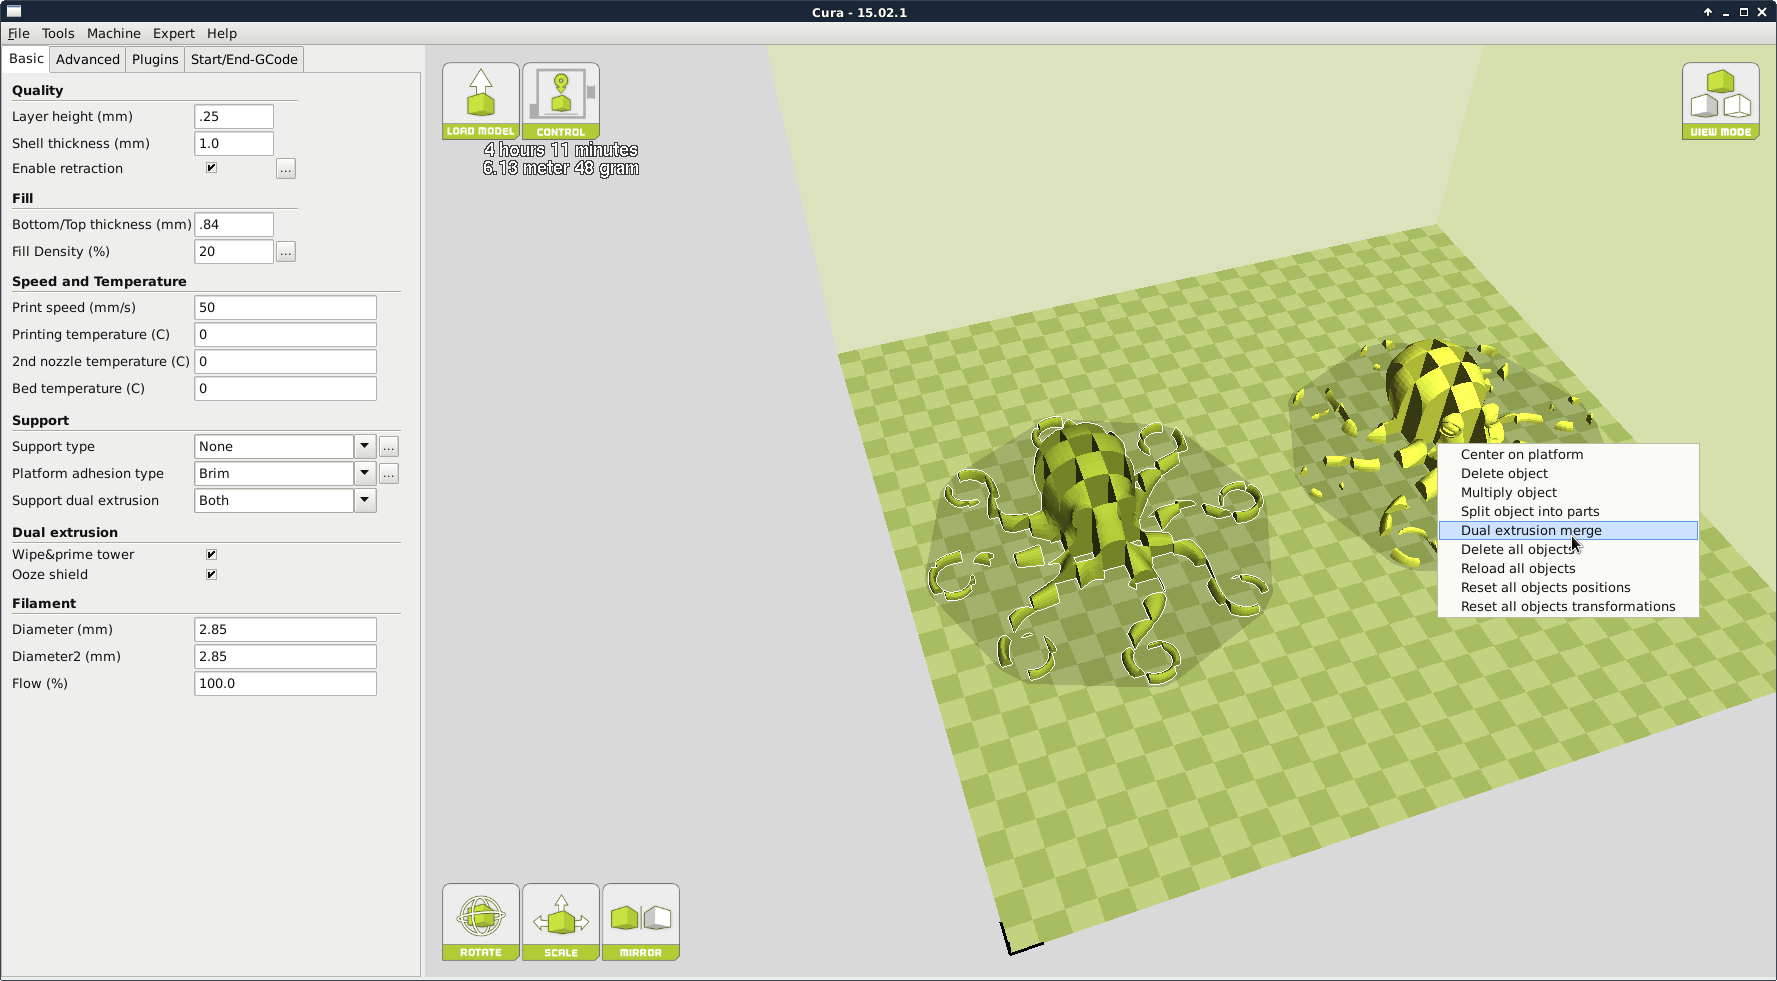
\includegraphics[keepaspectratio=true,angle=0,height=0.4\textheight,width=1.0\textwidth]{PreMerge.png}
\caption{Before Merge}
\label{fig:Before Merge}
\end{figure}

\subsection{Setting Dual Temps}
\index{Setting Dual Temps}
After your object has been merged as intended, you will need to set the individual temperatures for each print head. Open the Control Box as normal a normal print. In order to switch between which hot end you are heating, you will need to manually enter \texttt{T0} to set temps for the rear hot end, and \texttt{T1} to set temps for the front hot end. \texttt{The Bed temp can be set from either T0 or T1}. Once both print heads and the bed has reached temperature, go ahead and hit \texttt{Print.}

If you have any questions or would like some tips using your dual extruder, reach out to your fellow forum users at \texttt{http://Forum.LulzBot.com}.
